\documentclass[cn,11pt]{elegantbook}

\title{我的19岁}
\subtitle{电子设计大赛}

\author{余阳(Reyunn)}
\institute{武汉理工大学电子科技协会}
\date{\today}
\version{1.1.0}

\extrainfo{不争不抢,努力努力再努力。 --- 余阳}

\logo{logo.png}
\cover{cover.jpg}

\begin{document}

\maketitle
\tableofcontents


\mainmatter
\hypersetup{pageanchor=true}

\chapter{我的电赛经历}

我的19岁,很累。这一年在程序员的圈子里流行着996ICU的说法,但是这一年的我却过着8107的生活,每天早上8点到实验室,晚上10点离开,一周工作7天。并没有人强迫我这么做,但是我相信“强迫自己优秀,然后骄傲的生活”。在此说明,此文的写作时间始于2019年7月30日,此文并不是一个胜利者的经验分享会,而是为了纪念自己两年的付出及这两年的嵌入式开发。同时我想如果仅仅写自己的经历,那么一定没有人愿意阅读,为了使这篇文章的受众面更广一些,而第二部分是有关STM32单片机的分享,在第三部分则是我在这一年电赛经历的记录,最后的内容是我对大学不可回避的一些议题的讨论。总的来说这篇文章的前半部分是纪念我的奋斗岁月,而中间部分则是希望经验的传承,后半部分则是胡说八道。

我的相关联系方式:
\begin{itemize}
\item 个人博客:\href{http://reyunn.cn/}{http://reyunn.cn/}
\item Github 网址:\href{https://github.com/Reyunn/}{https://github.com/Reyunn/}
\item 邮件:\email{Reyunn@yandex.com}
\end{itemize}

\section{热血、迷茫}

提到我的大一生活,我想到的就是热血与迷茫。之所以迷茫是因为对未来的一无所知,之所以热血是因为想要摆脱迷茫,剥开云雾见青天。

导致这种状态的原因有两类:

\begin{enumerate}
\item 学校方面。开学过后学院组织了许多的经验分享会,所有的经验分享会大都是围绕着一个主题-"保研、考研"。但是刚入学的我,对老师、学长提供保研相关的数据并不太理解。那么我就迷茫了,保研的条件是什么?考研又是怎么一回事呢?……为此也立下了很多热血的flag,我要努力保研!我要保去华科!……

\begin{lstlisting}
“每个人的大学生活开始都是迷茫的,但是要尽快走出这段迷茫”。 -- 某位学长
\end{lstlisting}

\item 慕课方面。在课余生活经常看一些慕课,不可避免的接触到一些培训机构,他们大多宣传是的一些“读书无用论”,鼓吹“技术至上”。我因此迷茫,考研还是就业?学习什么技术?现在看来这对我既有利更有害,“利”在我提前接触到了一些企业更想要我们学习的技术(比如Java),“弊”在使自己忽略了基础学科的学习。

\begin{lstlisting}
“企业看中的不是你的专业,而是你的专长”。 -- 某培训机构
\end{lstlisting}
\begin{remark}
	以上两句引言,如有错误,欢迎指正,如帮助到你,不胜荣幸!
\end{remark}
\end{enumerate}

我想这一年我的电赛准备之路,也是热血与迷茫的。先说说热血,在大一上的学期末,自己并没有着急回家,选择留下来参加某校外机构的培训班,开始接触STC51单片机,大一下开学后每周六也去上相关课程。并在学期末有幸通过了学院实验室的招新考试,同时参加了实验室的暑假培训,培训的第一阶段从放假后到7月底,培训的第二阶段则是8月中旬开始的STM32相关的培训,虽然在此期间并没有掌握好STM32单片机,但是也为其学习开了个头。而迷茫在于,自己知道自己在准备电赛,但是电赛题目类型、题目的种类则是一无所知的。

\begin{figure}[htbp]
\centering

\includegraphics[width=\textwidth]{me1.jpg}
\caption{ 长江边跨年 }
\end{figure}

\section{自负、努力}

对大二上学期我的评价是一个贬义词,一个褒义词。正如之前所说的我的学习受到了培训机构的影响,在我之学到了一些皮毛时,我却沾沾自喜,说了一些不该说的话,做了一些不该做的事,现在看来当时的我是自负且幼稚。可以说是一叶障目,不见泰山。然而我还是想用努力来评价这个学期。也就是这个学期我有了8107的作息时间,风雨无阻,把实验室当家。

这个学期的电赛经历,我认为自己只配的上自负。其一:学习的方向偏向于应用方面,而忽略了STM32的学习。其二:对待校电子电工实验室的任务不重视,从而被劝退。所以,给大家一句忠告:一定要重视基础学科的学习!包括高数、模电、复变等。

\section{方向、两难}

对于大二下学期我认为摆在我面前的就是方向选择的问题,以及两难的处境。争取保研、准备考研、参加工作?准备电赛还是另寻它路?我想在最后一部分,就这些议题做谈谈我的看法。

在受到蓝桥杯失利以及涂劲豪与陈同凯的鼓励这双重影响下我也再次选择准备电赛。

为了参加电赛的第一步就是通过校赛初赛.为此我选择了最有效的途径,就是用什么学什么。在校赛的电源类的题目,STM32用到的其实就是ADC、PWM与PID控制算法。我一边参考学长留下来的代码,一边跟着B站学习,以不错的效果通过了初赛,通过初赛后我们在校实验室也就重新获得了座位。

为了参加电赛的第二步就是通过校赛的复赛与决赛。复赛是三天两夜的持续性工作,因为初赛至复赛的周期很短,在此期间我也没办法再多学习什么内容,所以复赛真的做的很糟糕。而决赛只有一个上午,题目相对简单( 信号、电源结合的题目 ) ,且以硬件为主,做的效果不能说差。

为了参加电赛的最后一步就是术业有专攻的学习,仅从电源类的角度来说,编程最重要的就是3点:ADC、SPWM、PID,逐一击破即可。(第三部分有更细致的分享)

在准备比赛的过程中,我想过要放弃。因为自己半路参加电赛,要准备的东西太多了,但是“我不去想自己是否能取得成功,既然选择远方,便只顾风雨兼程”。

\section{致谢}
文章写到这,离比赛还有一周。对比赛的结果,自己已经不太在乎了。如果自己未能取得好的名次,还希望大家不要以成败论英雄,不要因此而认为这篇文章就是垃圾。自己能走到这一步,要感谢的人有很多。包括我的队友、指导老师、家人、电子科技协会、室友……

\chapter{STM32的学习}

在你阅读这个部分的时候,我希望你对STM32的寄存器及库函数的开发方式有所了解。而这一部分的主要内容则是基于HAL库 和 Cube MX的开发方式。本来我有计划写一个部分介绍STC51单片机,但是这两者重复部分太多,所以最终仅保留STM32部分,并对其做更细致的探讨。


如果你学过STC51,你一定知道STC51操作是极其方便的。如果你学过STM32的库函数,你一定知道STM32操作是极其繁琐的。传统的库函数开发方式,将太多时间花费在各种东西的初始化上。同时,如果你学过STM32F1、STM32F3、STM32F4的话,你会发现对于不同型号的STM32在使用库函数的开发方式下,他的初始化流程也是不一样的,这也是传统开发方式的一种弊端。\textbf{而Cube MX + HAL库开发的方式,则是省去了初始化的部分,让开发人员将更多的精力放在业务的处理!}但是寄存器及库函数的开发方式也是有必要学习的,因为Cube MX也可能存在Bug,如果你对寄存器及库函数不了解那你会很被动。


如有错误,欢迎指正,如有帮助,不胜荣幸!

\section{GPIO}

GPIO(英语:General-purpose input/output),通用型之输入输出的简称,其接脚可以供使用者由程控自由使用,PIN脚依现实考量可作为通用输入(GPI)或通用输出(GPO)或通用输入与输出(GPIO)

\subsection{GPIO 8种工作模式}

GPIO\_Mode\_AIN 模拟输入

GPIO\_Mode\_IN\_FLOATING 浮空输入

GPIO\_Mode\_IPD 下拉输入

GPIO\_Mode\_IPU 上拉输入

GPIO\_Mode\_Out\_OD 开漏输出

GPIO\_Mode\_Out\_PP 推挽输出

GPIO\_Mode\_AF\_OD 复用开漏输出

GPIO\_Mode\_AF\_PP 复用推挽输出


\subsection{应用总结}

1、上拉输入、下拉输入可以用来检测外部信号;例如,按键等;

2、浮空输入模式,由于输入阻抗较大,一般把这种模式用于标准通信协议的I2C、USART的接收端;

3、普通推挽输出模式一般应用在输出电平为0和3.3V的场合。而普通开漏输出模式一般应用在电平不匹配的场合,如需要输出5V的高电平,就需要在外部一个上拉电阻,电源为5V,把GPIO设置为开漏模式,当输出高阻态时,由上拉电阻和电源向外输出5V电平。

4、对于相应的复用模式(复用输出来源片上外设),则是根据GPIO的复用功能来选择,如GPIO的引脚用作串口的输出(USART/SPI/CAN),则使用复用推挽输出模式。如果用在I2C、SMBUS这些需要线与功能的复用场合,就使用复用开漏模式。

5、在使用任何一种开漏模式时,都需要接上拉电阻。

\subsection{Cube MX相关配置}

\subsubsection{选择引脚类型}
 
	GPIO\_Input-输入引脚	GPIO\_Output-输出引脚
\begin{figure}[htbp]
	\centering
	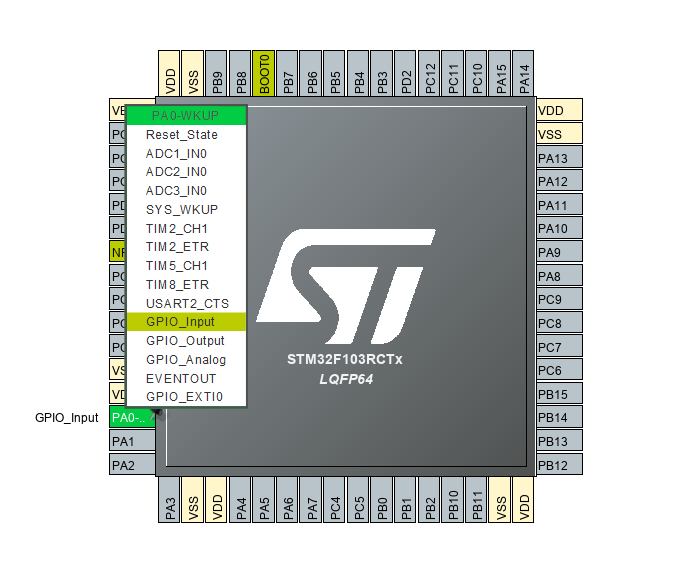
\includegraphics[width=0.6\textwidth]{gpio_1.png}
	\caption{选择引脚类型 \label{fig:scatter}}
\end{figure}

\subsubsection{配置引脚}

对于输入引脚,可以配置的就是GPIO Pull-up/Pull-down。这分别对应的就是Pull-up( 输入上拉 )与Pull-down ( 输入下拉)。

Pull-up:输入上拉就是把电位拉高,比如拉到Vcc。上拉就是将不确定的信号通过一个电阻嵌位在高电平。电阻同时起到限流的作用。弱强只是上拉电阻的阻值不同,没有什么严格区分。

Pull-down:输入下拉就是把电压拉低,拉到GND。与上拉原理相似。

简单的说,如果你希望你的引脚平时处于高电平用于检测低电平,你就使用Pull-up。如果你希望你的引脚平时处于低电平用于检测高电平,你就使用Pull-down。

\begin{figure}[htbp]
	\centering
	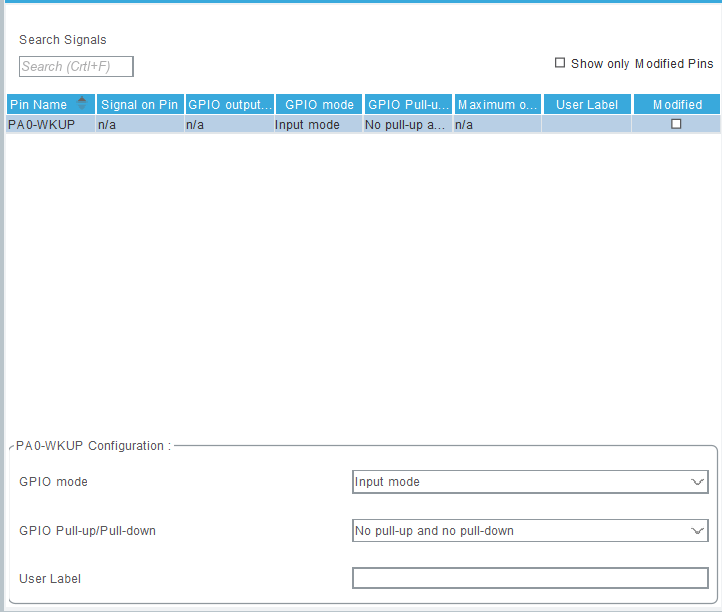
\includegraphics[width=0.6\textwidth]{gpio_2.png}
	\caption{配置输入引脚 \label{fig:scatter}}
\end{figure}

\newpage


对于输出引脚,比输入多了更多的配置:

GPIO output level -> 初始化输出电平 

GPIO mode -> 输出方式 -> 开漏或推挽输出

GPIO Pull-up/Pull-down -> 上拉或下拉输出

Maximum output speed 选中GPIO管脚的速率

\emph{选中GPIO管脚的速率}

I/O口的输出模式下,有3种输出速度可选(Low - 2MHz、Medium - 10MHz、High - 50MHz),这个速度是指I/O口驱动电路的响应速度而不是输出信号的速度,输出信号的速度与程序有关(芯片内部在I/O口 的输出部分安排了多个响应速度不同的输出驱动电路,用户可以根据自己的需要选择合适的驱动电路)。通过选择速度来选择不同的输出驱动模块,达到最佳的噪声控制和降低功耗的目的。高频的驱动电路,噪声也高,当不需要高的输出频率时,请选用低频驱动电路,这样非常有利于提高系统的EMI性能。当然如果要输出较高频率的信号,但却选用了较低频率的驱动模块,很可能会得到失真的输出信号。

举个栗子:

1、USART串口,若最大波特率只需115.2k,那用2M的速度就够了,既省电也噪声小。

2、I2C接口,若使用400k波特率,若想把余量留大些,可以选用10M的GPIO引脚速度。

3、SPI接口,若使用18M或9M波特率,需要选用50M的GPIO的引脚速度。

\begin{figure}[htbp]
	\centering
	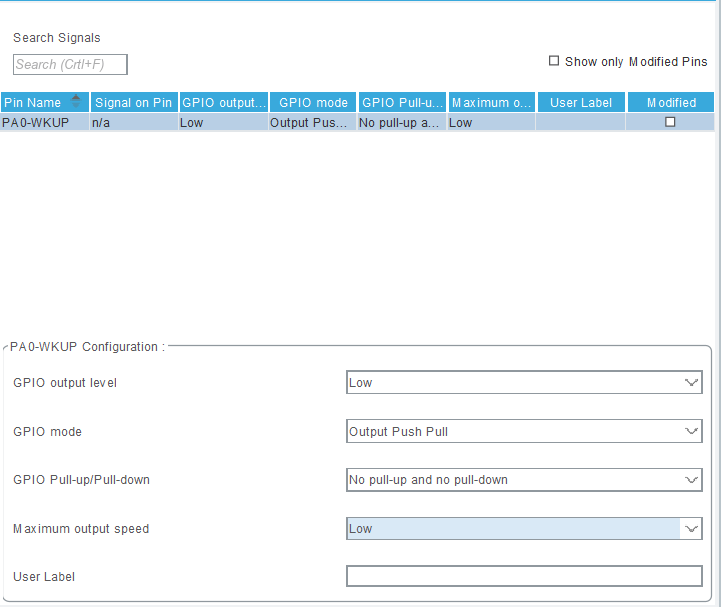
\includegraphics[width=0.6\textwidth]{gpio_3.png}
	\caption{配置输出引脚 \label{fig:scatter}}
	
\end{figure}

\newpage

\subsection{编写业务代码}

\subsubsection{初始化及重置相关}

\lstset{  language=C}
\begin{lstlisting}
//初始化引脚
void  HAL_GPIO_Init(GPIO_TypeDef  *GPIOx, GPIO_InitTypeDef *GPIO_Init); 
 //重置引脚
void  HAL_GPIO_DeInit(GPIO_TypeDef  *GPIOx, uint32_t GPIO_Pin);
\end{lstlisting}

\subsubsection{IO口操作相关}

\lstset{language=C}
\begin{lstlisting}

//读取电平状态
GPIO_PinState HAL_GPIO_ReadPin(GPIO_TypeDef *GPIOx, uint16_t GPIO_Pin);
//设置引脚状态
void HAL_GPIO_WritePin(GPIO_TypeDef *GPIOx, uint16_t GPIO_Pin, GPIO_PinState PinState);
//转换引脚状态
void HAL_GPIO_TogglePin(GPIO_TypeDef *GPIOx, uint16_t GPIO_Pin);
//锁定引脚状态
HAL_StatusTypeDef HAL_GPIO_LockPin(GPIO_TypeDef *GPIOx, uint16_t GPIO_Pin);

\end{lstlisting}

同时HAL库帮我定义好了GPIO\_PIN\_RESET与GPIO\_PIN\_SET,代表着1(高电平)、0(低电平)。


\subsection{User Label}

对于任意引脚,它都有这么一个选项。我想告诉你这个选项特别特别好用!这个选项简单的说就是它帮你在main.h中生成define语句。但是对于HAL库编程,main.h会被用户的每个模块调用,也就是这些define语句的作用域几乎是全局。


\begin{figure}[htbp]
	\centering
	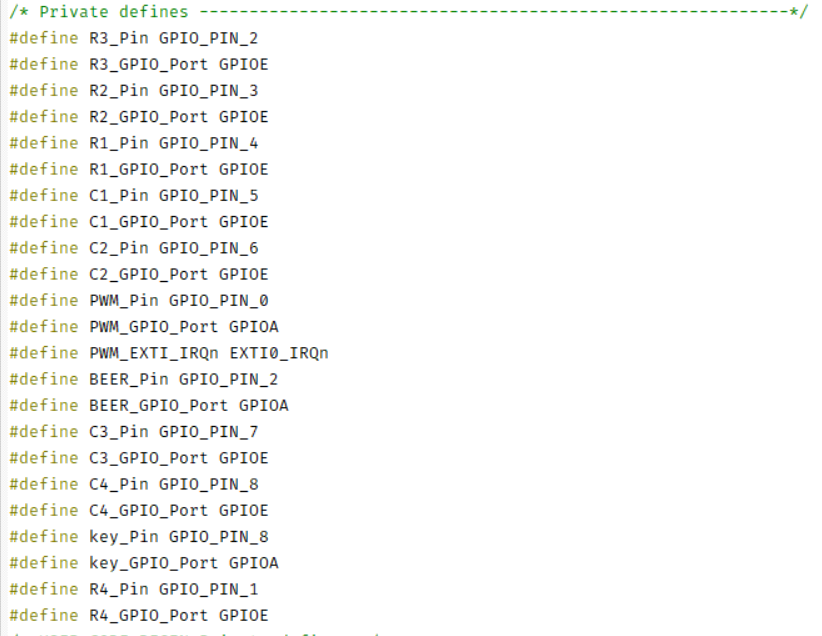
\includegraphics[width=0.6\textwidth]{gpio_4.png}
	\caption{Cube MX生成的define语句 \label{fig:scatter}}
\end{figure}

举个例子让你感受一下,在一次开发中,我使用PA0来作为输出引脚。如果随着开发的继续PA0被迫要用于其他功能,那么你该怎么办?那你必须使用另外一个引脚( 假设是PB1) 来替代它。

如果你没有配置User Label选项,那你的代码中可能大量的充斥着
\lstset{  language=C}
\begin{lstlisting}
HAL_GPIO_WritePin(GPIOA, GPIO_PIN_0, GPIO_PIN_RESET);//将PA0引脚状态改为低电平
HAL_GPIO_WritePin(GPIOA, GPIO_PIN_0, GPIO_PIN_SET);//将PA0引脚状态改为高电平
\end{lstlisting}

然后你又需要用PB1来代替PA0,那你就需要将整个代码中有关PA0的GPIOA改成GPIOB,将GPIO\_PIN\_0改成GPIO\_PIN\_1。这会导致巨大的工作量,并且容易出错。

那么我们来看看使用了User Label会带来什么变化,使用User Label 把他取名R1。那你的代码中充斥着的不在是 HAL\_GPIO\_WritePin(GPIOA, GPIO\_PIN\_0, GPIO\_PIN\_RESET),而是HAL\_GPIO\_WritePin(R1\_GPIO\_Port, R1\_Pin, GPIO\_PIN\_RESET)。当遇到PA0被迫要用于其他功能,你只需要把PB1的User Label 取名为R1后,代码不需要做丝毫改变。

在我的开发中,这个应用最典型的两个例子就是“矩阵键盘”和“ADS1256”的开发。用矩阵键盘来举例,需要用到8个引脚。

\begin{figure}[htbp]
	\centering
	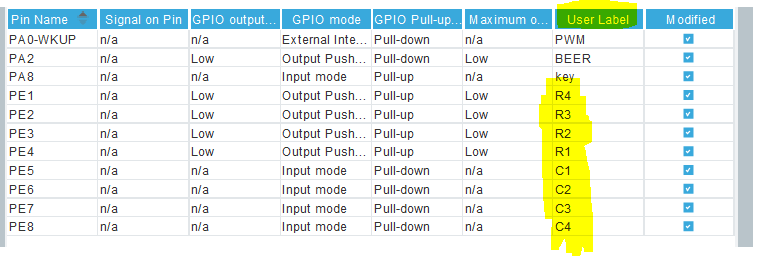
\includegraphics[width=1.0\textwidth]{gpio_5.png}
	\caption{Cube MX的配置\label{fig:scatter}}
\end{figure}

我的矩阵键盘中的代码全是由R1-R4、C1-C4组成,所以在各这个代码的复用性极其强,无论是换引脚还是换单片机型号,我只需要在Cube MX中配置一下,就可以马上投入使用。

\begin{figure}[htbp]
	\centering
	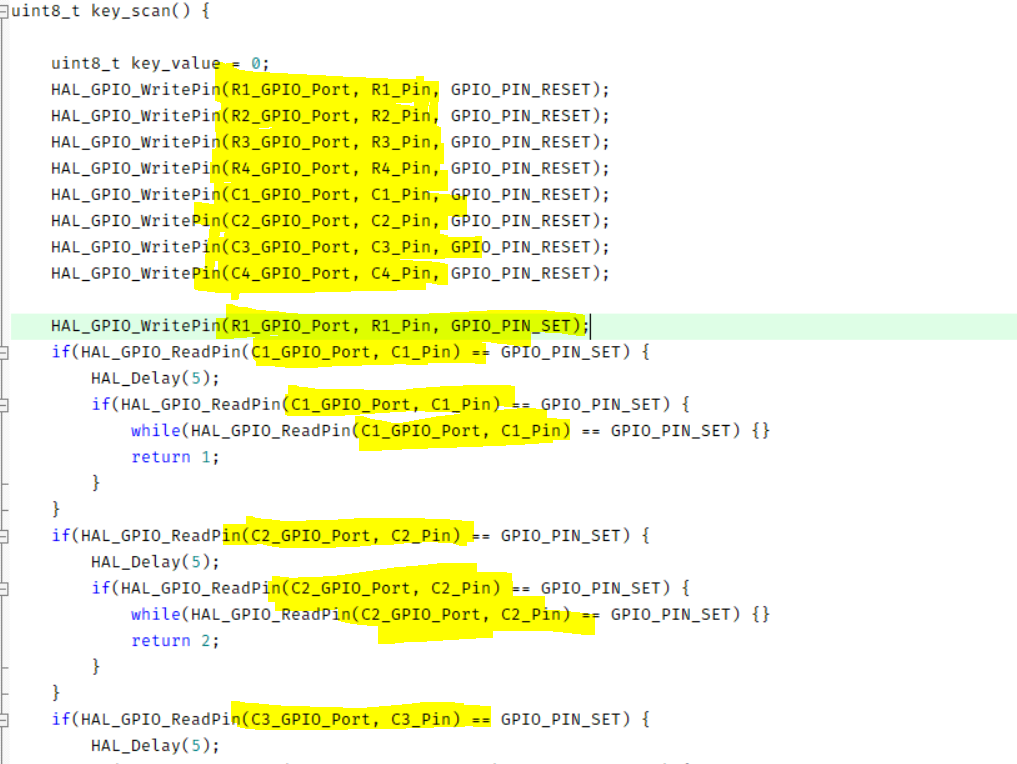
\includegraphics[width=1.0\textwidth]{gpio_6.png}
	\caption{矩阵键盘代码截图\label{fig:scatter}}
\end{figure}

\section{串口通信}

串口通信(Serial Communications)的概念非常简单,串口按位(bit)发送和接收字节。

\subsection{UART 与 USART}

UART:通用异步收发传输器(Universal Asynchronous Receiver/Transmitter),通常称作UART。它将要传输的资料在串行通信与并行通信之间加以转换。作为把并行输入信号转成串行输出信号的芯片,UART通常被集成于其他通讯接口的连结上。

USART:(Universal Synchronous/Asynchronous Receiver/Transmitter)通用同步/异步串行接收/发送器,USART是一个全双工通用同步/异步串行收发模块,该接口是一个高度灵活的串行通信设备。
\subsection{Cube MX相关配置}

\subsubsection{初始化引脚}

Mode : 

Asynchronous : 异步, 整个过程,不会阻碍发送者的工作。

Synchronous : 同步, 同步信息一旦发送,发送者必须等到应答,才能继续后续的行为。

Single Wire : 单总线,半双工。

\begin{figure}[htbp]
	\centering
	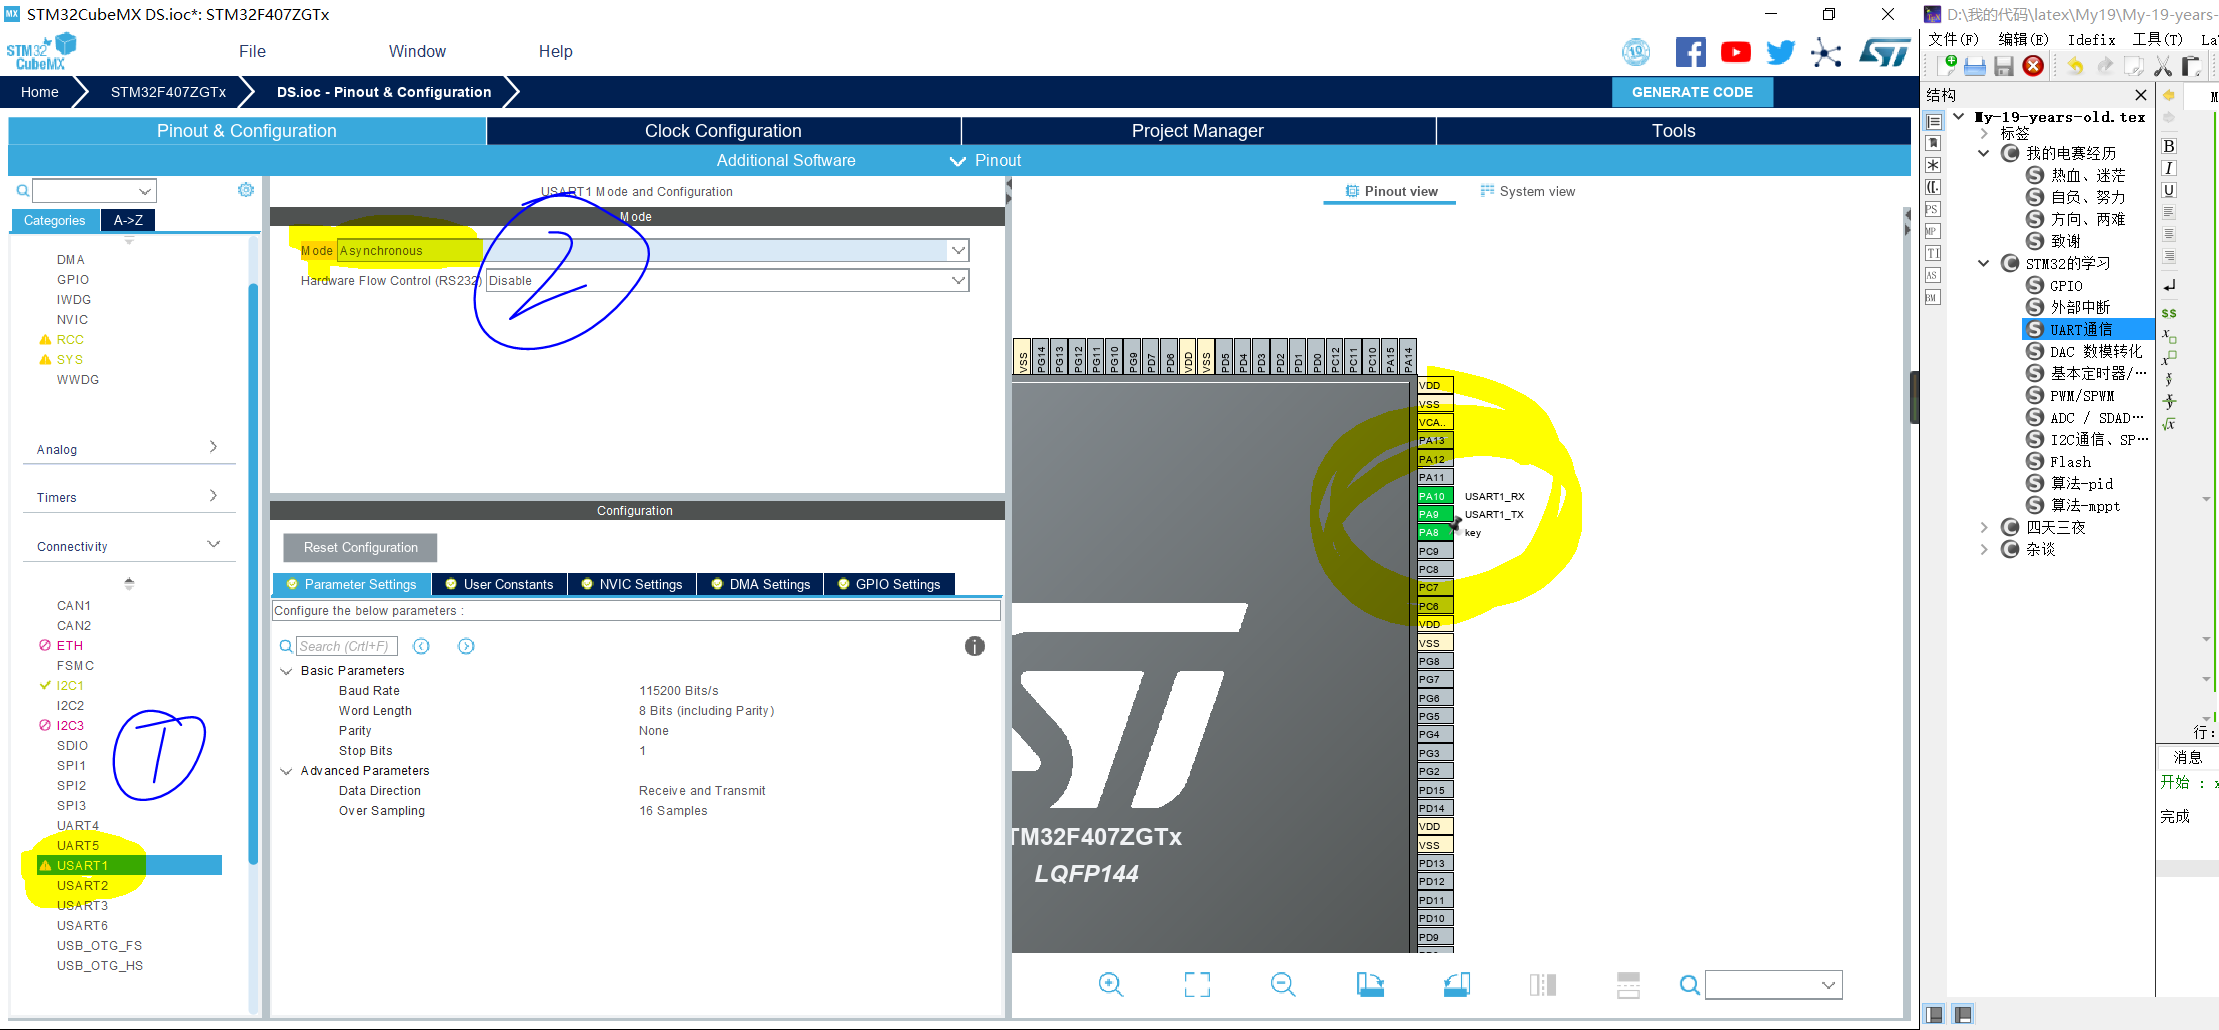
\includegraphics[width=1.0\textwidth]{uart_1.png}
	\caption{使能引脚\label{fig:scatter}}
\end{figure}

\subsubsection{配置引脚}

Baud Rate: 波特率,波特率表示每秒钟传送的码元符号的个数,是衡量数据传送速率的指标,它用单位时间内载波调制状态改变的次数来表示。对于串口最重要的就是波特率,常用的波特率为115200与9600。

Wrod Length : 数据长

Parity : 奇偶校验 -> 无、奇校验、偶校验

Stop : 停止位

以上的配置与需要通信双方完全配对

\begin{figure}[htbp]
	\centering
	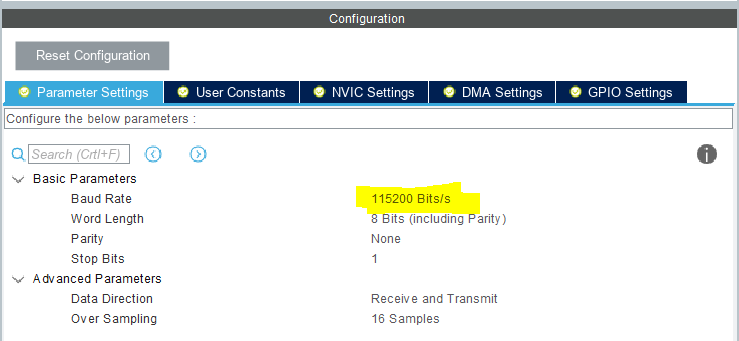
\includegraphics[width=1.0\textwidth]{uart_2.png}
	\caption{配置引脚\label{fig:scatter}}
\end{figure}

\newpage

\subsection{编写逻辑代码}

\lstset{  language=C}
\begin{lstlisting}
//发送数据
HAL_StatusTypeDef HAL_UART_Transmit(UART_HandleTypeDef *huart, uint8_t *pData, uint16_t Size, uint32_t Timeout);
//接收数据
HAL_StatusTypeDef HAL_UART_Receive(UART_HandleTypeDef *huart, uint8_t *pData, uint16_t Size, uint32_t Timeout);
//发送中断
HAL_StatusTypeDef HAL_UART_Transmit_IT(UART_HandleTypeDef *huart, uint8_t *pData, uint16_t Size);
//接收中断
HAL_StatusTypeDef HAL_UART_Receive_IT(UART_HandleTypeDef *huart, uint8_t *pData, uint16_t Size);
//使用DMA发送
HAL_StatusTypeDef HAL_UART_Transmit_DMA(UART_HandleTypeDef *huart, uint8_t *pData, uint16_t Size);
//使用DMA接收
HAL_StatusTypeDef HAL_UART_Receive_DMA(UART_HandleTypeDef *huart, uint8_t *pData, uint16_t Size);
//DMA暂停
HAL_StatusTypeDef HAL_UART_DMAPause(UART_HandleTypeDef *huart);
//DMA恢复
HAL_StatusTypeDef HAL_UART_DMAResume(UART_HandleTypeDef *huart);
//DMA停止
HAL_StatusTypeDef HAL_UART_DMAStop(UART_HandleTypeDef *huart);
\end{lstlisting}
就我目前的学习来看HAL并没有对同步通信的方式做拓展,所以上述都是关于UART的函数。

\subsection{printf重定向}
在Private includes中引入:
\begin{lstlisting}
#include <stdio.h>
\end{lstlisting}

在USER CODE BEGIN 0添加:
\lstset{  language=C}
\begin{lstlisting}
int fputc(int ch, FILE *f){
	uint8_t temp[1] = {ch};
	HAL_UART_Transmit(&huart1, temp, 1, 2);//huart1需要根据你的配置修改
	return ch;
}

\end{lstlisting}
然后你就可以在任意地方使用printf语句方便的输出你想要的内容。

\subsection{Log信息格式}

\subsubsection{格式1}

参考目前主流嵌入式、安卓等输出方式:

\lstset{ language=C}
\begin{lstlisting}
[日志级别] 文件名 : 日志信息
//例:[info] main.c : init ok!
//例: [debug] adc.c : adc_getvalue -> 3.3v
\end{lstlisting}


\subsubsection{格式2}

参考Java日志框架的输出方式:

\lstset{ language=C}
\begin{lstlisting}
[         文件名] 日志级别 : 日志信息
//例:[       main] info : init ok!
//例: [       adc] debug : adc_getvalue -> 3.3v
\end{lstlisting}

\subsection{条件编译}

说到这里我还想向大家介绍一下条件编译。因为在进行单片机开发的过程中,会需要大量的Log信息,但是在开发结束时,你又不想它一直打印( 这会拖慢单片机的速度 )。所以我提出我的办法:

在头文件中添加:
\lstset{  language=C}
\begin{lstlisting}
#define Log 1 // 打印Log信息,不想打印时改为0即可
\end{lstlisting}

再把.c文件中将所有的printf包裹上 \#if Log  与 \#endif:

\lstset{ language=C}
\begin{lstlisting}
#if Log 
printf("[info]main.c:init!\r\n");
#endif
\end{lstlisting}

下面截选mppt算法中条件编译的使用:
\begin{figure}[htbp]
	\centering
	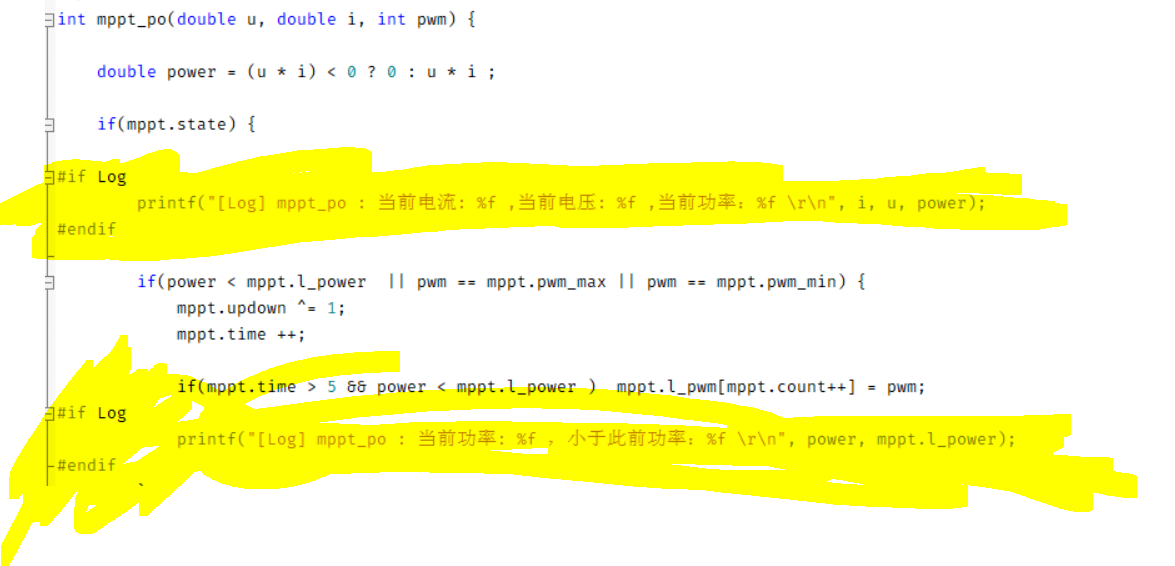
\includegraphics[width=1.0\textwidth]{uart_3.png}
	\caption{条件编译在代码中的使用\label{fig:scatter}}
\end{figure}

\subsection{可变参数宏}

关于这个内容,是我在阅读国内某云物联网模块源码是发现并学习的。

\begin{figure}[htbp]
	\centering
	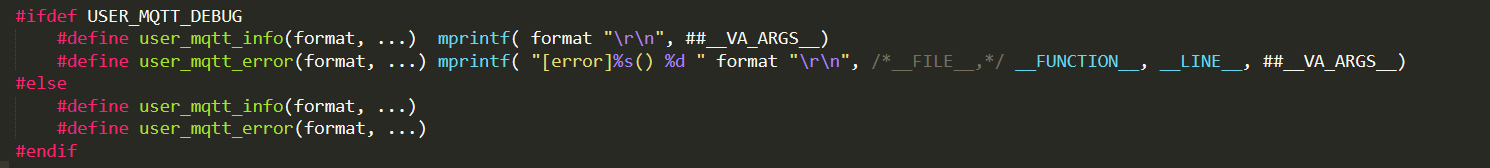
\includegraphics[width=1.0\textwidth]{uart_4.png}
	\caption{源码学习\label{fig:scatter}}
\end{figure}

我觉得这个解决方案比之前提到的条件编译强100倍,甚至让我感觉到以前的做法多么的愚蠢。这种方法不仅达到了代码的格式化,同时也完成了条件编译。

在此分享我的设计:

\begin{lstlisting}
#ifdef USER_MAIN_DEBUG
#define user_main_printf(format, ...)  printf( format "\r\n", ##__VA_ARGS__)
#define user_main_info(format, ...)  printf("[\tmain]info:" format "\r\n", ##__VA_ARGS__)
#define user_main_debug(format, ...) printf("[\tmain]debug:" format "\r\n", ##__VA_ARGS__)
#define user_main_error(format, ...) printf("[\tmain]error:" format "\r\n",##__VA_ARGS__)
#else
#define user_main_printf(format, ...)
#define user_main_info(format, ...)
#define user_main_debug(format, ...)
#define user_main_error(format, ...)
#endif
\end{lstlisting}

当我需要打印串口信息的时候,define一个USER\_MAIN\_DEBUG,在我不需要时将其注释。

\subsection{个性化输出}

1、借助下面的网站设计自己的字符

\href{http://patorjk.com/software/taag/}{http://patorjk.com/software/taag/}
\begin{figure}[htbp]
	\centering
	
\includegraphics[width=1.0\textwidth]{uart_5.png}
	\caption{字符组成的reyunn\label{fig:scatter}}
\end{figure}	

2、编写代码

先逐行复制输入

\begin{figure}[htbp]
	\centering
	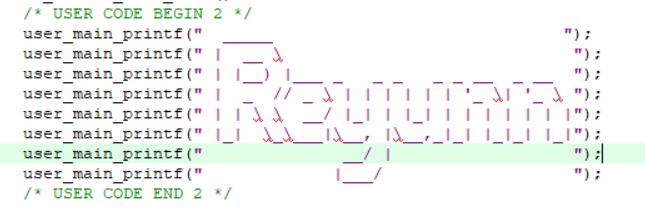
\includegraphics[width=0.6\textwidth]{uart_6.png}
	\caption{逐行复制输入\label{fig:scatter}}
\end{figure}	

再用转义字符修补错误

\begin{figure}[htbp]
	\centering
	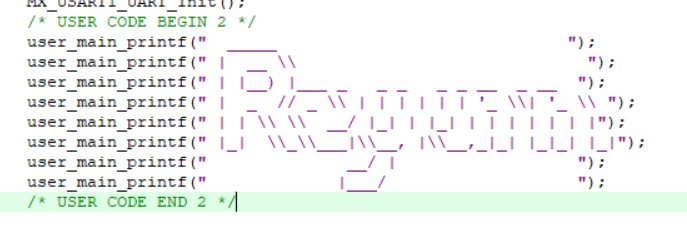
\includegraphics[width=0.6\textwidth]{uart_7.png}
	\caption{转义字符修补错误\label{fig:scatter}}
\end{figure}


3、串口助手看效果

\begin{figure}[htbp]
	\centering
	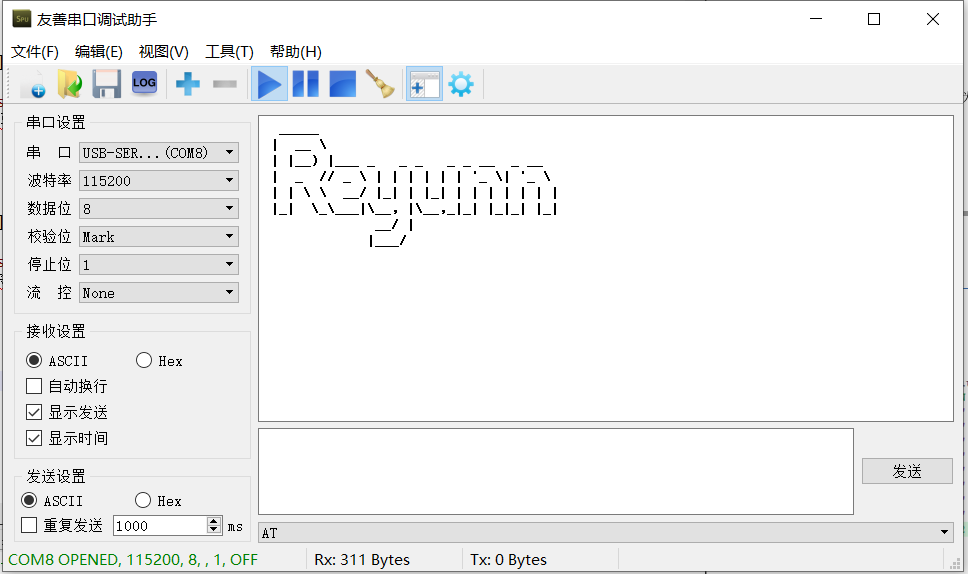
\includegraphics[width=1.0\textwidth]{uart_8.png}
	\caption{打印信息效果\label{fig:scatter}}
\end{figure}

\subsection{串口中断}
1、Cube MX中开启中断
\begin{figure}[htbp]
	\centering
	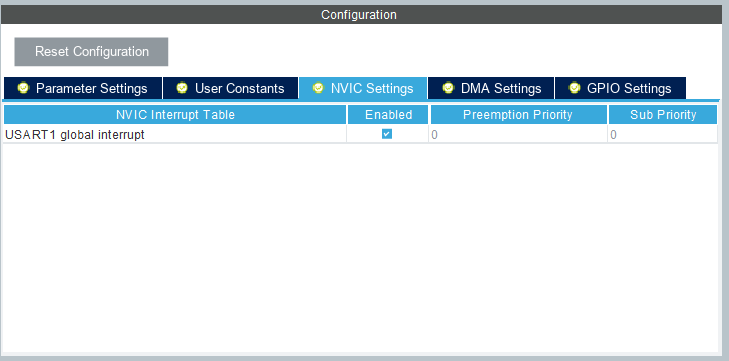
\includegraphics[width=0.9\textwidth]{uart_9.png}
	\caption{开启中断\label{fig:scatter}}
\end{figure}


2、在USER CODE BEGIN 2 中打开串口中断

\lstset{ language=C}
\begin{lstlisting}
HAL_UART_Receive_IT(&huart1, temp, 1);
\end{lstlisting}

3、在USER CODE BEGIN 4 中实现回调函数


\lstset{ language=C}
\begin{lstlisting}
void HAL_UART_RxCpltCallback(UART_HandleTypeDef *huart) {
	if(huart -> Instance == huart1.Instance ) {
		...//业务代码
	}
}
\end{lstlisting}


\section{外部中断}
外部中断是单片机实时地处理外部事件的一种内部机制。当某种外部事件发生时,单片机的中断系统将迫使CPU暂停正在执行的程序,转而去进行中断事件的处理;中断处理完毕后.又返回被中断的程序处,继续执行下去。
\subsection{Cube MX相关配置}

\subsubsection{初始化引脚}

如果你想使用PA1作为外部中断的接收引脚,那么你只需要点击PA1,在点击它对应的GPIO\_EXTIx
\begin{figure}[htbp]
	\centering
	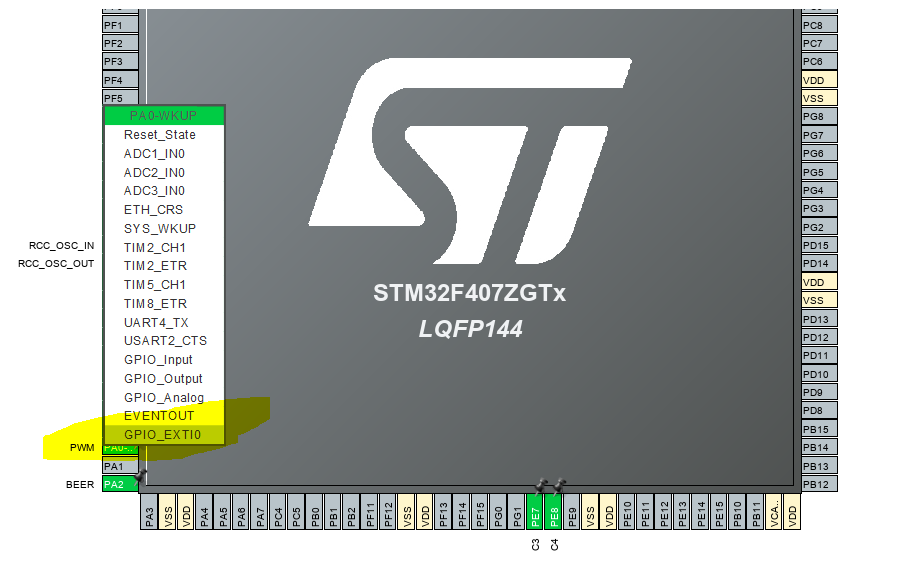
\includegraphics[width=1.0\textwidth]{exti_1.png}
	\caption{使能引脚\label{fig:scatter}}
\end{figure}

\subsubsection{使能中断}

\begin{figure}[htbp]
	\centering
	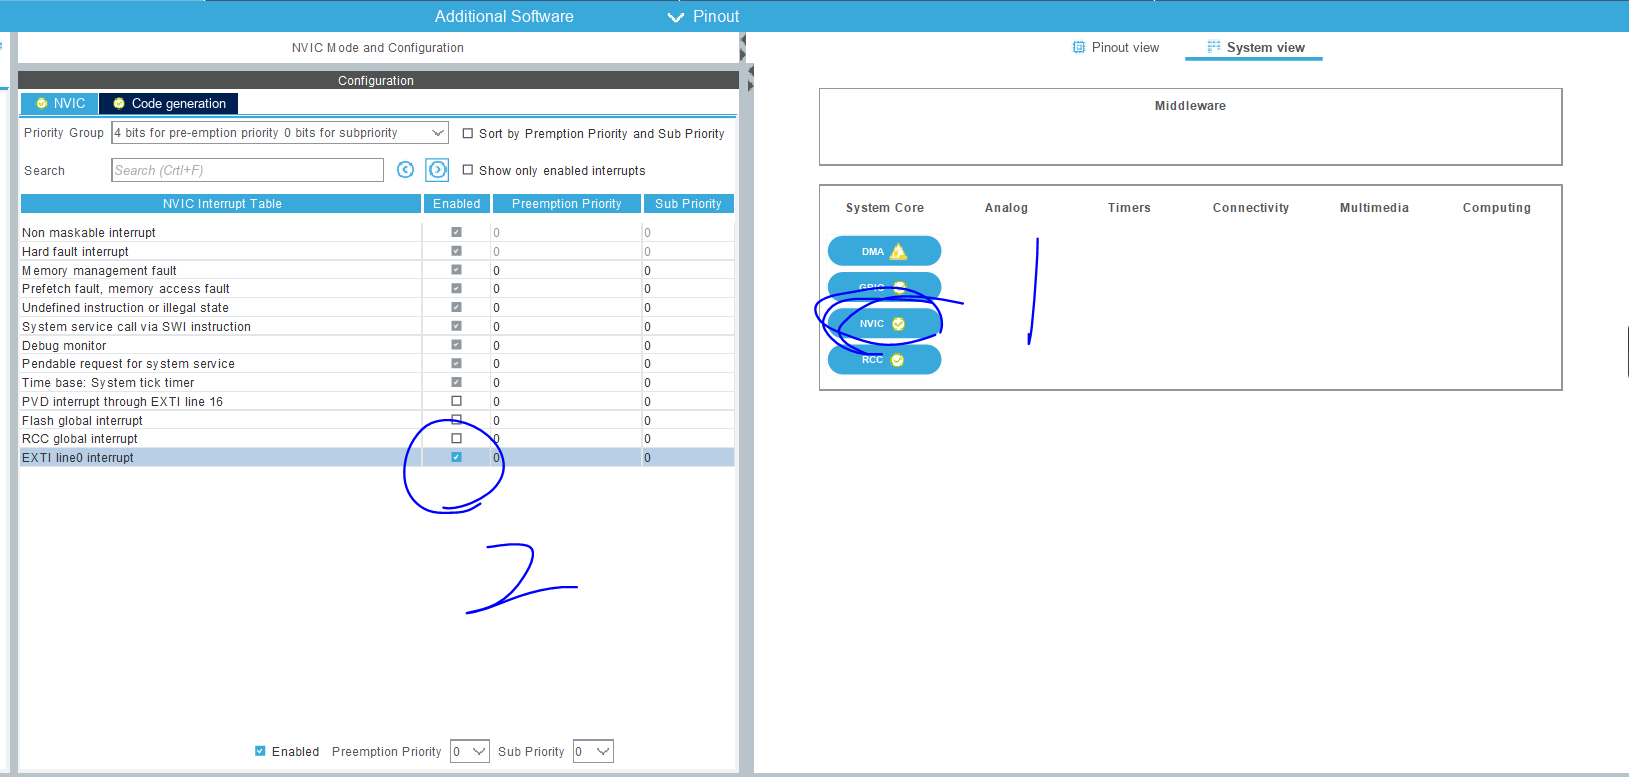
\includegraphics[width=1.0\textwidth]{exti_3.png}
	\caption{使能中断\label{fig:scatter}}
\end{figure}

\newpage

\subsubsection{配置引脚}

这个地方与此前不同的地方在于GPIO mode。

External Interrupt Mode with Rising edge trigger detection//上升沿触发

External Interrupt Mode with Falling edge trigger detection//下降沿触发

External Interrupt Mode with Rising/Falling edge trigger detection//上升沿或下降沿触发

\begin{figure}[htbp]
	\centering
	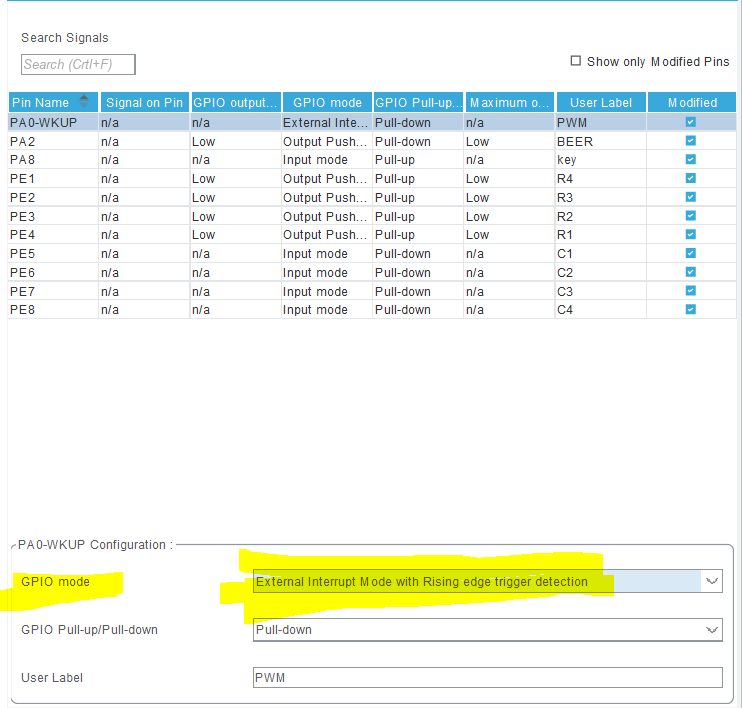
\includegraphics[width=0.6\textwidth]{exti_2.png}
	\caption{配置引脚\label{fig:scatter}}
\end{figure}


\subsection{编写逻辑代码}

在main.c中的USER CODE BEGIN 4编程范围内添加外部中断的回调函数:

\newpage

\lstset{  language=C}
\begin{lstlisting}
void HAL_GPIO_EXTI_Callback(uint16_t GPIO_Pin) {
	if(GPIO_Pin == PWM_Pin) {
		...//业务代码
	}
}
\end{lstlisting}

\subsection{测量pwm频率}


在我平时的学习中没有太多的使用外部中断,但是在最后的电赛中却巧妙的使用了它。

当时的情况是我们需要测量一个PWM的频率,我的解决办法是这样的:

当有上升沿的时候,就进入外部中断将pwm\_value的值+1。it is clear that "1s钟上升沿的次数就是pwm的频率"。所以当我要用pwm的频率时,我就先将pwm\_value置0,再延时1s,最后再使用pwm\_value。当然这并不是我最终的代码,因为你读到这里还有很多的内容没有学习,往后的定时器章节将介绍它的滤波算法。

\lstset{  language=C}
\begin{lstlisting}

int pwm_value =0 ;

int main(){

	while (1){
		pwm_value = 0; // pwm_value置0
		HAL_Delay(1000); // 延时1s
		printf("[\tmain]info:pwm_value=%d\r\n",pwm_value); // 读取pwm_value
	}

}

/**
  * @brief 外部中断的回调函数
  * @param GPIO_Pin 触发中断的引脚
  * @retval None
  */
void HAL_GPIO_EXTI_Callback(uint16_t GPIO_Pin) {
	if(GPIO_Pin == PWM_Pin) { // 判断触发引脚是否是定义的引脚
		pwm_value++; 
	}
}

\end{lstlisting}

\newpage


\section{时钟树}
说到STM32,必然逃不开时钟树。但是时钟树要展开讲的话会很麻烦,而且我也不一定讲的好。但是我想告诉你的是:通常我们会让单片机的频率( 决定单片机的处理速度)提到最大,再进行其他分频操作。

原谅我技术有限,所以我想分享的关于时钟树的就是小小的一点:

\subsection{使能外部时钟源}

\begin{figure}[htbp]
	\centering
	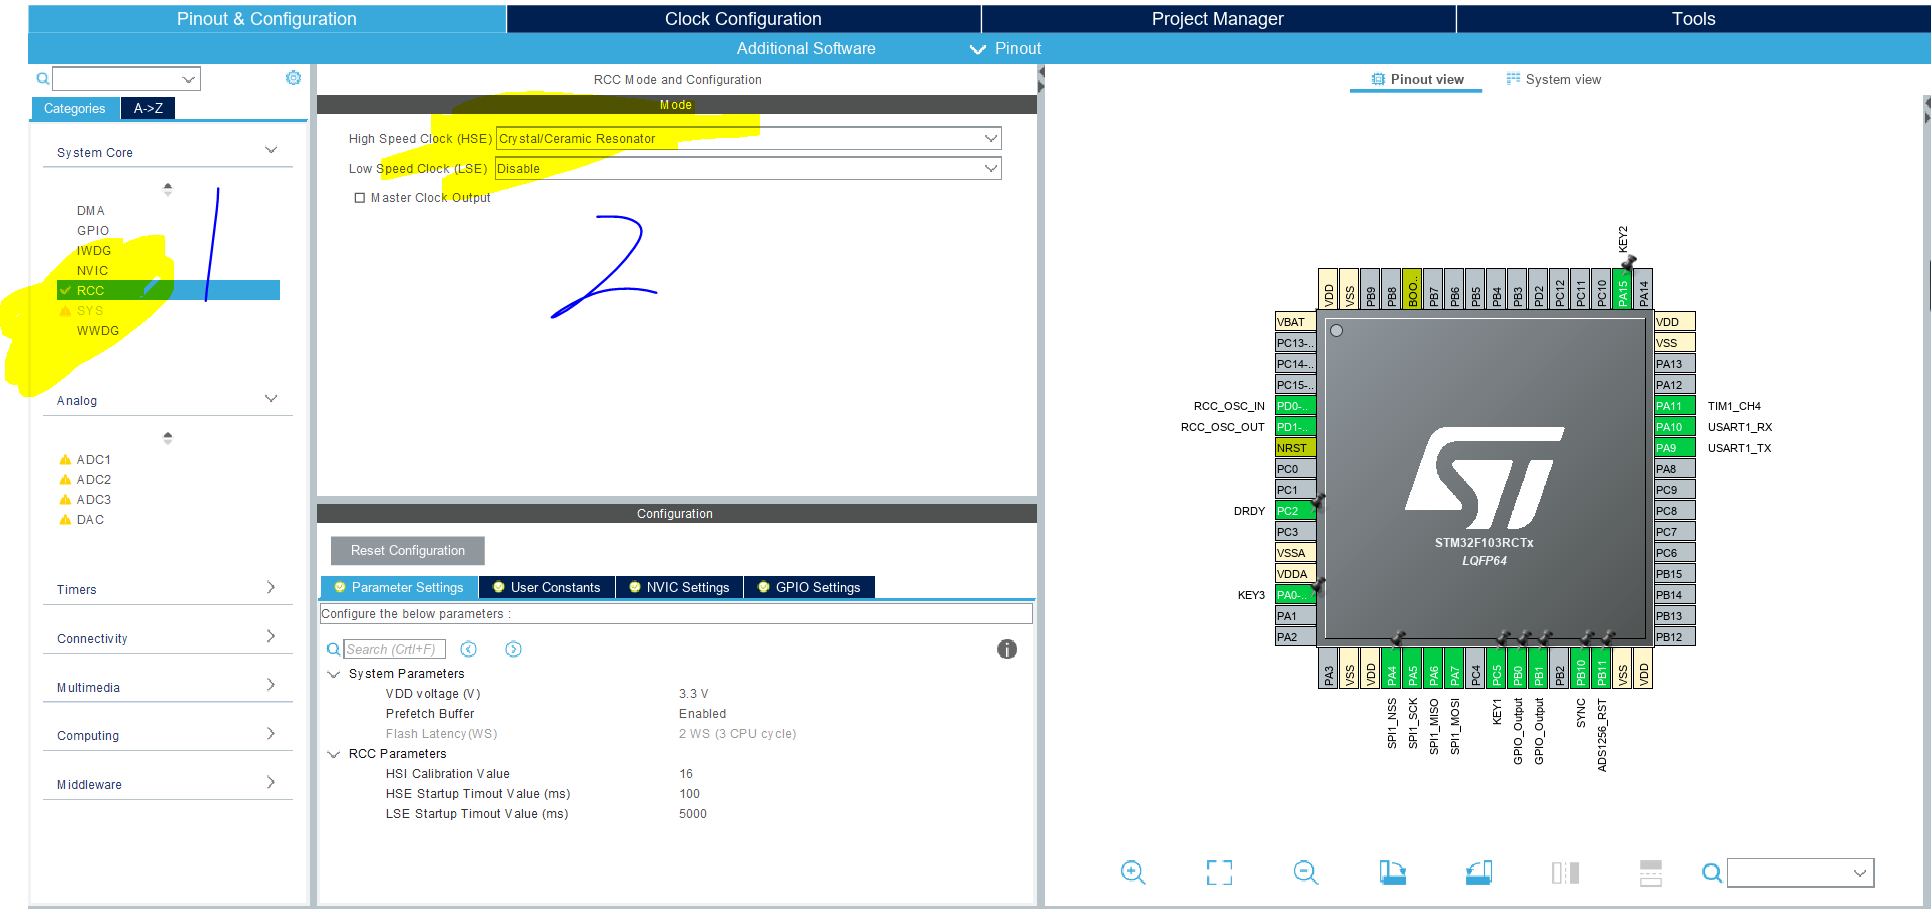
\includegraphics[width=1.0\textwidth]{rcc1.png}
	\caption{使能外部时钟源 \label{fig:scatter}}
\end{figure}

\subsection{将频率调至最大}

不同单片机的最大运行频率是不同的,例如stm32f103为72M而stm32f407为84M。

\begin{figure}[htbp]
	\centering
	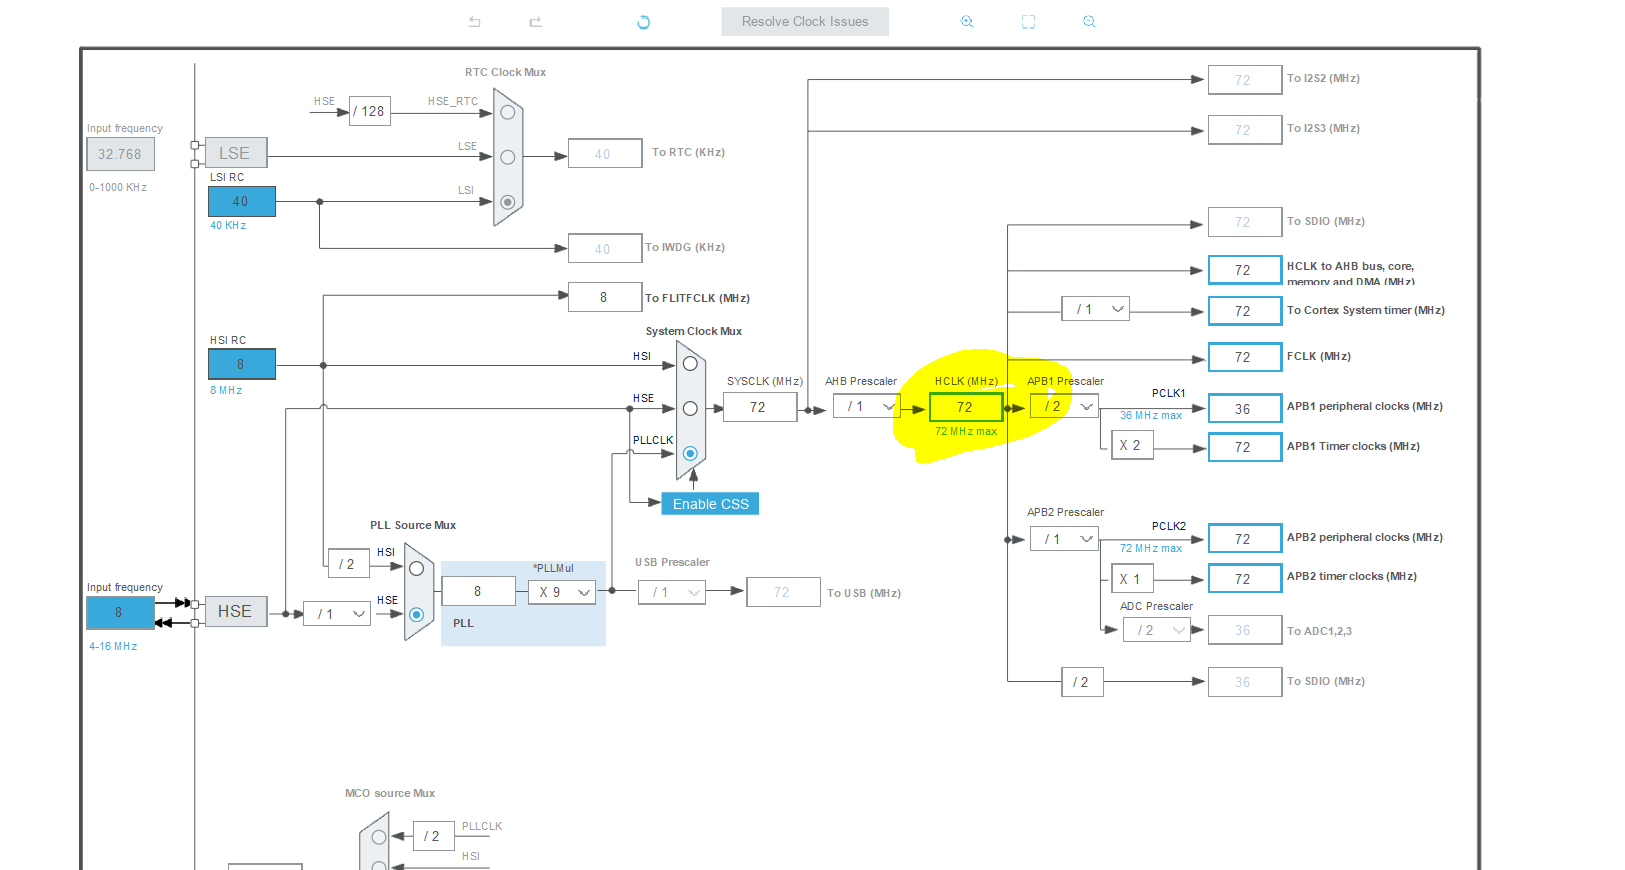
\includegraphics[width=1.0\textwidth]{rcc2.png}
	\caption{将频率调至最大 \label{fig:scatter}}
\end{figure}


\subsection{按需分频}


\begin{figure}[htbp]
	\centering
	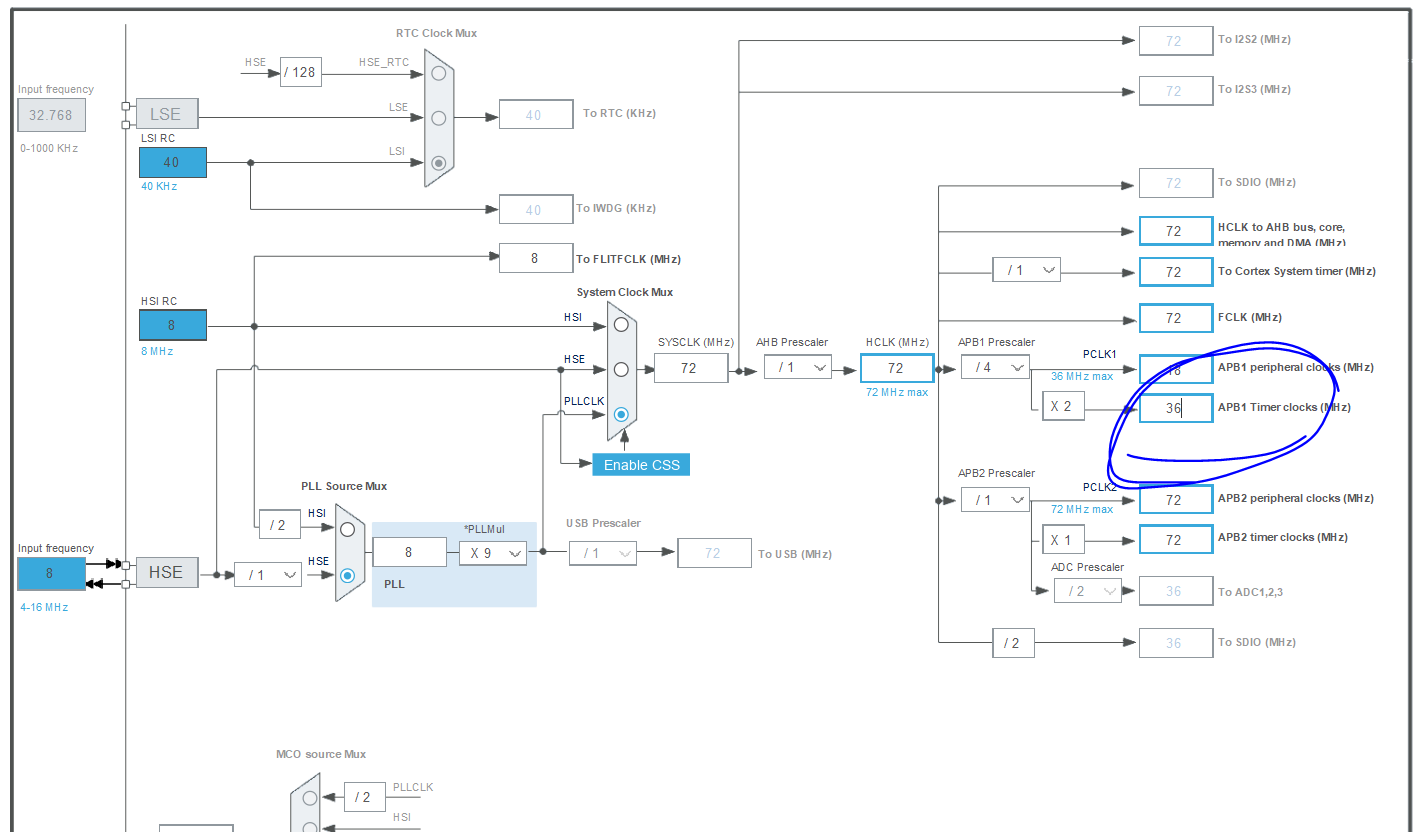
\includegraphics[width=0.9\textwidth]{rcc3.png}
	\caption{按需分频 \label{fig:scatter}}
\end{figure}

\section{定时器}
分享完时钟树的部分,接下来就是和它最紧密的定时器了。定时器最基本的内容就是定时产生中断了:
\subsection{Cube MX相关配置}
\subsubsection{配置定时器时钟}


如之前所示,将定时器的时钟设为72M。
\begin{figure}[htbp]
	\centering
	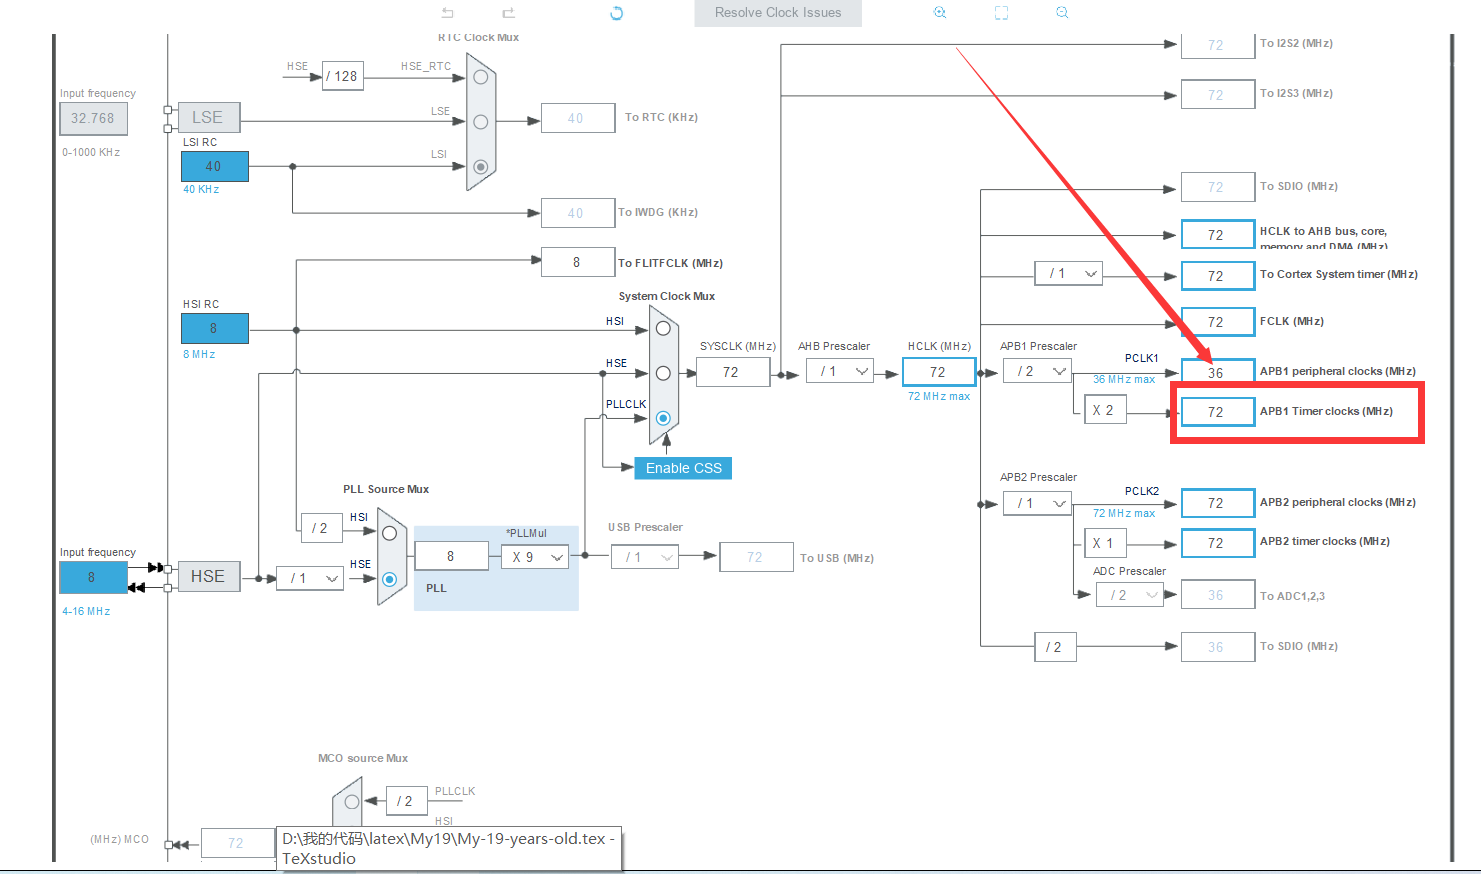
\includegraphics[width=0.8\textwidth]{tim_1.png}
	\caption{配置定时器频率 \label{fig:scatter}}
\end{figure}


\subsubsection{选择时钟源}

选择内部时钟

\begin{figure}[htbp]
	\centering
	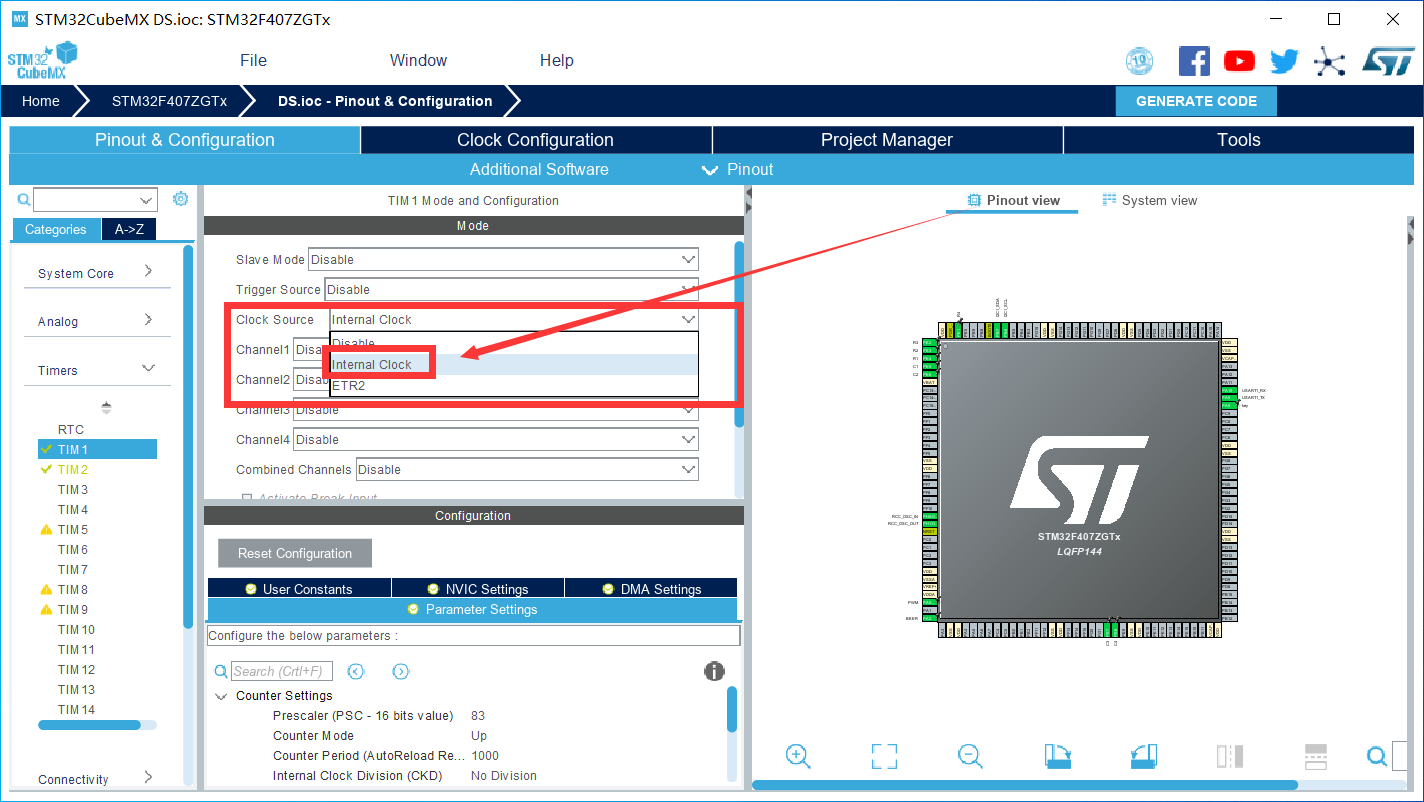
\includegraphics[width=1.0\textwidth]{tim_2.png}
	\caption{选择时钟源 \label{fig:scatter}}
\end{figure}

\subsubsection{配置定时器}

定时器的配置主要有两个:定时时间与是否重装定时器。

定时频率 = 定时器时钟 / ( 预分频 +1) /(  计数值 + 1 )  Hz。
  
定时时间 = 1 /  定时频率 s。

\begin{figure}[htbp]
	\centering
	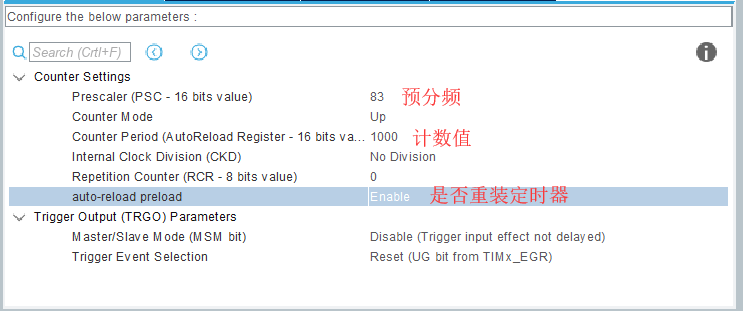
\includegraphics[width=1.0\textwidth]{tim_3.png}
	\caption{配置定时器 \label{fig:scatter}}
\end{figure}

\subsubsection{开启中断 - 基本定时器}

勾选Enabled框即可。

\begin{figure}[htbp]
	\centering
	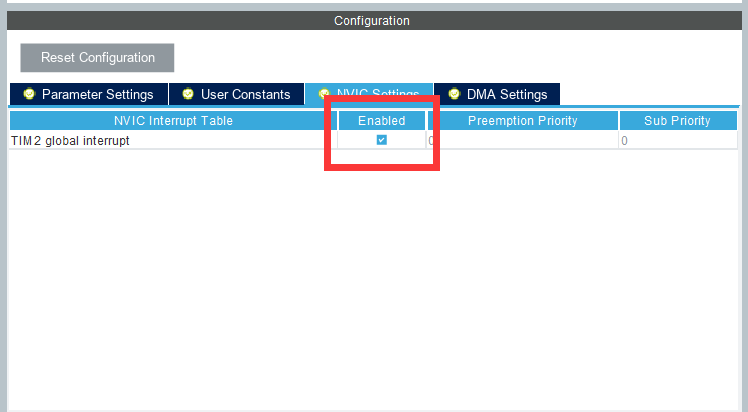
\includegraphics[width=1.0\textwidth]{tim_4.png}
	\caption{开启中断 \label{fig:scatter}}
\end{figure}

\newpage

\subsubsection{开启中断 - 高级定时器}

勾选TIM X update interrupt 后的 Enabled框即可。

\begin{figure}[htbp]
	\centering
	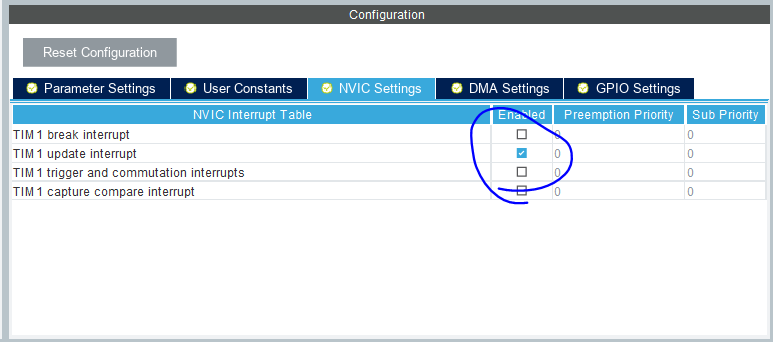
\includegraphics[width=1.0\textwidth]{tim_5.png}
	\caption{开启中断 \label{fig:scatter}}
\end{figure}

\subsection{编写业务代码}

\lstset{language=C}
\begin{lstlisting}
int main(){

	HAL_TIM_Base_Start_IT(&htim1); //定时器1使能
	HAL_TIM_Base_Start_IT(&htim2); //定时器2使能
	...

}

void HAL_TIM_PeriodElapsedCallback(TIM_HandleTypeDef *htim) {

	if (htim->Instance == htim1.Instance) {
		...//定时器1中断业务
	}

	else if(htim-> Instance == htim2.Instance) {
		 ...//定时器2中断业务
	}
	...
}
\end{lstlisting}

\subsection{平滑滤波}

在这里我想在介绍定时器的另一种用法:平滑滤波。绝大部分人的滤波算法都是用的时候,多次采样再滤波。但是我希望让采样值在另一个“线程”一直滤波,而在我需要他的时候,直接取它的值即可。记得之前我描述过用外部中断实现的测量pwm波的频率,接下我想分享一下用定时器对其进行滤波。
\lstset{language=C}
\begin{lstlisting}
/* 定时器2配置为0.1s触发一次中断 */
/**
  * @brief 定时器中断的回调函数
  * @param htim 触发中断的定时器
  * @retval None
  */
void HAL_TIM_PeriodElapsedCallback(TIM_HandleTypeDef *htim) {
	if(htim-> Instance == htim2.Instance) {
		pwm_sum += pwm_value * 10;    //pwm_sum累加
		pwm_sum -= pwm_avg;           //pwm_sum减去上次的平均值
		pwm_avg = pwm_sum * 1.0 / 5;  //更新pwm的平均值
		pwm_value_final = pwm_avg;    //pwm_value_final的值即为当前pwm的频率
		pwm_value = 0;                //将pwm_value清空,重新计数
	}
}
/**
  * @brief 外部中断的回调函数
  * @param GPIO_Pin 触发中断的引脚
  * @retval None
  */
void HAL_GPIO_EXTI_Callback(uint16_t GPIO_Pin) {
	if(GPIO_Pin == PWM_Pin) { // 判断触发引脚是否是定义的引脚
		pwm_value++; 
	}
}
\end{lstlisting}
当我们在任意时刻需要使用pwm的频率时,只需要使用pwm\_value\_final的值即可。



\section{PWM/SPWM}

脉冲宽度调制(PWM),是英文“Pulse Width Modulation”的缩写,简称脉宽调试。是利用微处理器的数字输出来对模拟电路进行控制的一种非常有效的技术。广泛应用在从测量、通信到功率控制与变换的许多领域中。

SPWM(Sinusoidal PWM)法是一种比较成熟的、使用较广泛的PWM法。冲量相等而形状不同的窄脉冲加在具有惯性的环节上时,其效果基本相同。SPWM法就是以该结论为理论基础,用脉冲宽度按正弦规律变化而和正弦波等效的PWM波形即SPWM波形控制逆变电路中开关器件的通断,使其输出的脉冲电压的面积与所希望输出的正弦波在相应区间内的面积相等,通过改变调制波的频率和幅值则可调节逆变电路输出电压的频率和幅值。

PWM和SPWM在电源的备战中是很有必要的。基础的恒流源、恒压源需要使用PWM的占空比及频率来达到数控的作用,往后的逆变则需要用到SPWM。那我就先从简单的PWM做分享,PWM输出其实是定时器的一种应用。那么配置定时器时钟与选择时钟源我就不再赘述了。就从使能PWM通道开始讲起。
\subsection{Cube MX相关配置-PWM}
\subsubsection{使能PWM通道}

在这里我将TIM2的Channel1设置为PWM输出通道(PWM Generation CHx正向 、PWM Generation CHxN反向 、 PWM Generation CHx CHxN一对互补pwm输出)

\begin{figure}[htbp]
	\centering
	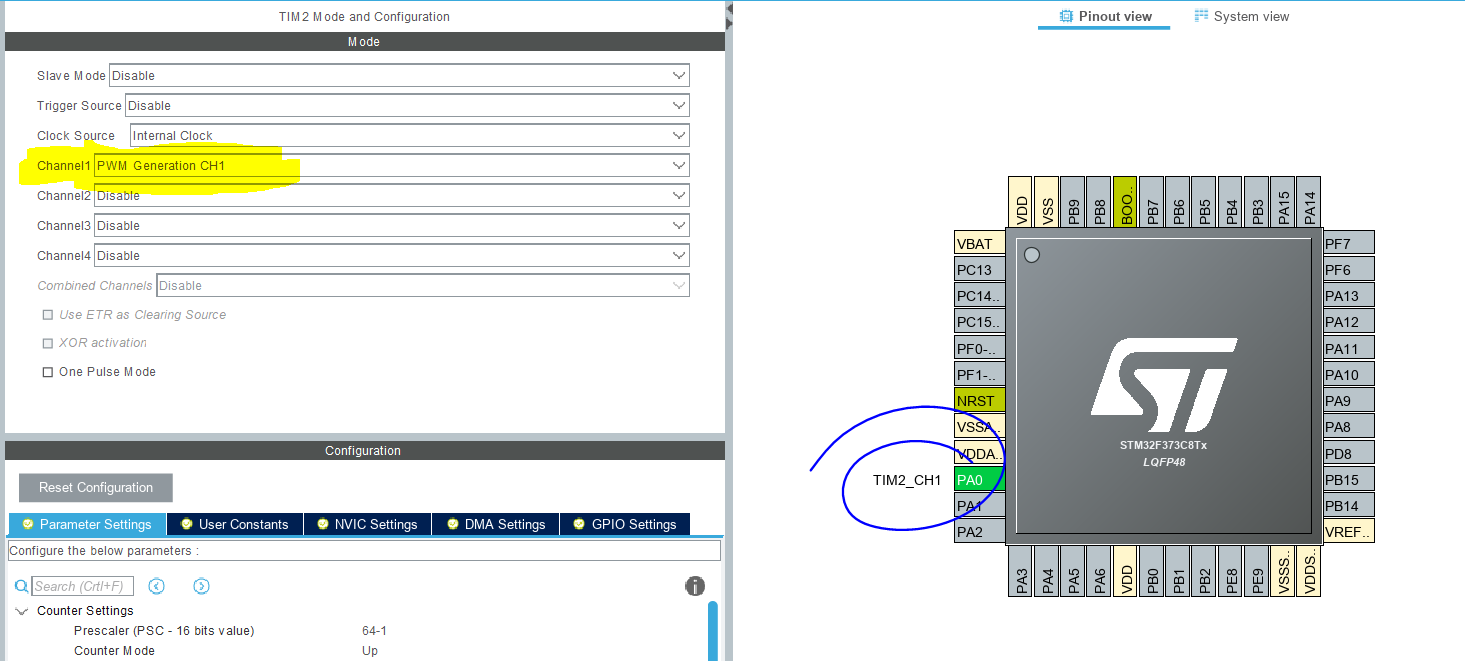
\includegraphics[width=1.0\textwidth]{pwm_1.png}
	\caption{使能PWM通道 \label{fig:scatter}}
\end{figure}


\subsubsection{配置频率及占空比}

频率 = 定时器时钟 / ( Prescaler预分频 + 1) /  (   Counter Period计数值 + 1)  Hz

占空比 = Pulse ( 对比值 )  / ( C ounter Period计数值  ) \%


\begin{figure}[htbp]
	\centering
	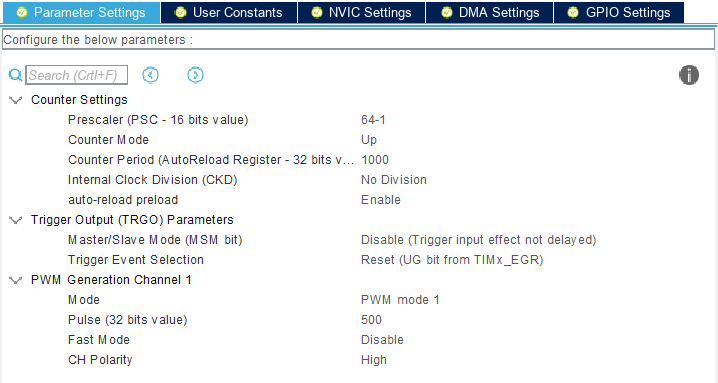
\includegraphics[width=1.0\textwidth]{pwm_2.png}
	\caption{配置频率及占空比 \label{fig:scatter}}
\end{figure}

\subsection{编写业务代码-PWM}

\lstset{language=C}
\begin{lstlisting}
// 使能timx的通道y
HAL_TIM_PWM_Start(&htimx,TIM_CHANNEL_y); 
// 修改timx的通道y的pwm比较值为z,即修改占空比
__HAL_TIM_SET_COMPARE(&htimx, TIM_CHANNEL_y, z); 
\end{lstlisting}

pwm的输出是很简单的,但是因为定时器的频率是有上限的通常需要在频率和pwm的精细度两者之间做取舍。所以你想做电源,那么你可以了解一下STM32F334这款处理器,它拥有一个高分辨率定时器(HRTIM),能将定时器的频率倍频至4.096G。那你在频率和pwm的精细度两者都可以兼得。

\emph{SPWM其实就是在PWM的基础上,让PWM的占空比做正弦变化。}

\subsection{Cube MX相关配置-SPWM}


之前的PWM生成的操作不变,只需要开启一个新的定时器,配置完后需要开启定时器中断

\begin{figure}[htbp]
	\centering
	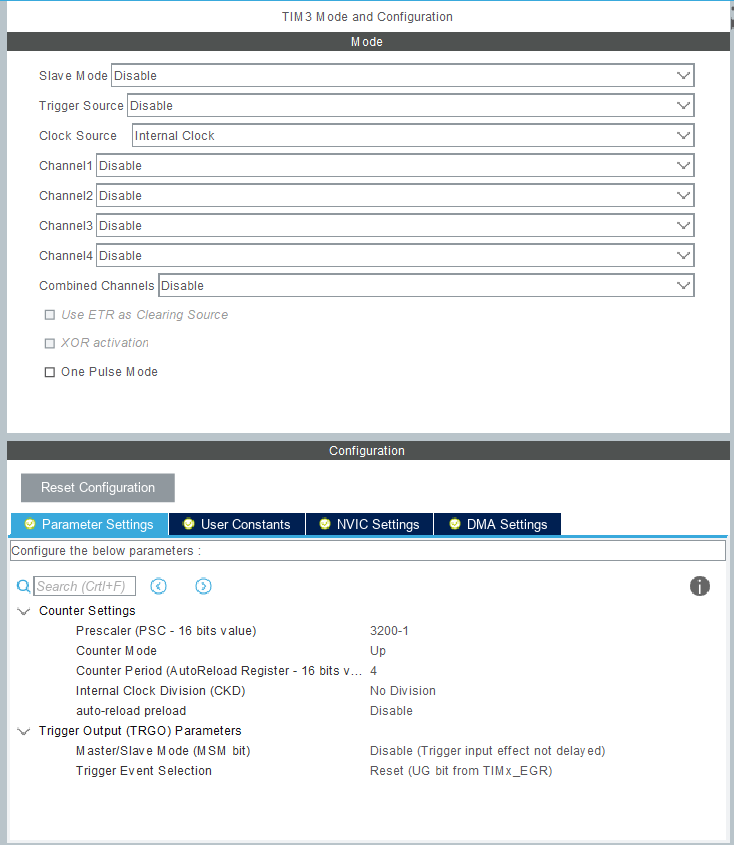
\includegraphics[width=0.6\textwidth]{spwm_1.png}
	\caption{开启一个新的定时器 \label{fig:scatter}}
\end{figure}
\newpage
\subsection{使用软件生成正弦向量表-SPWM}
SPWM 中值 = Pulse ( 对比值 ) /2

SPWM 幅值 = Pulse ( 对比值 ) /2

周内点数影响频率与正弦波精细度。周内点数越大,频率越小、正弦波精细度越高。

\begin{figure}[htbp]
	\centering
	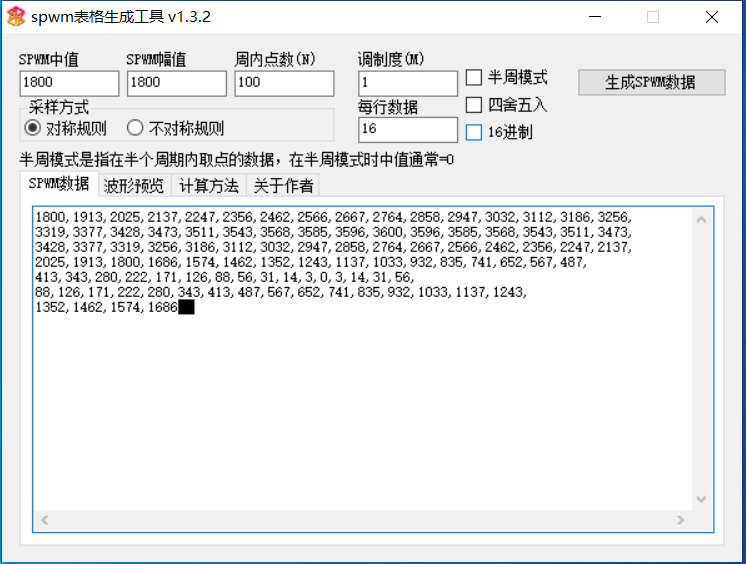
\includegraphics[width=0.6\textwidth]{spwm_2.png}
	\caption{使用软件生成正弦向量表 \label{fig:scatter}}
\end{figure}

\subsection{编写业务代码-SPWM}

\lstset{language=C}
\begin{lstlisting}
uint16_t sin[] = {
	1800,1913,2025,2137,2247,2356,2462,2566,2667,2764,
	2858,2947,3032,3112,3186,3256,3319,3377,3428,3473,
	3511,3543,3568,3585,3596,3600,3596,3585,3568,3543,
	3511,3473,3428,3377,3319,3256,3186,3112,3032,2947,
	2858,2764,2667,2566,2462,2356,2247,2137,2025,1913,
	1800,1686,1574,1462,1352,1243,1137,1033,932,835,
	741,652,567,487,413,343,280,222,171,126,
	88,56,31,14,3,0,3,14,31,56,
	88,126,171,222,280,343,413,487,567,652,
	741,835,932,1033,1137,1243,1352,1462,1574,1686
}

int main(){
	HAL_TIM_PWM_Start(&htimx,TIM_CHANNEL_y);  // 开启pwm输出
	HAL_TIM_Base_Start_IT(&htimz); //使能刚刚配置的定时器z
	while(1){
	}
}
/**
  * @brief 定时器中断的回调函数
  * @param htim 触发中断的定时器
  * @retval None
  */
void HAL_TIM_PeriodElapsedCallback(TIM_HandleTypeDef *htim){
	static int i = 0;
	if(++i == size)i = 0;
	if (htim->Instance == htim3.Instance){
		__HAL_TIM_SET_COMPARE(&htimx, TIM_CHANNEL_y,  sin[i]); //由向量表修改占空比
	}
}
\end{lstlisting}
对于做电源的同学来说,这个是必须要掌握的内容!


\section{ADC / SDADC / ADS 模数转化}

先介绍最简单的片上ADC,通常是12位,精度则为3.3/4096 v。

读取ADC的方式有很多:

 1、轮询 
 
 2、中断 
 
 3、DMA 
 
因为在实际开发中仅有轮询和DMA存在使用场景,所以在这里我仅介绍轮询和DMA的方式。

\subsection{Cube MX相关配置-轮询方式}

\begin{figure}[htbp]
	\centering
	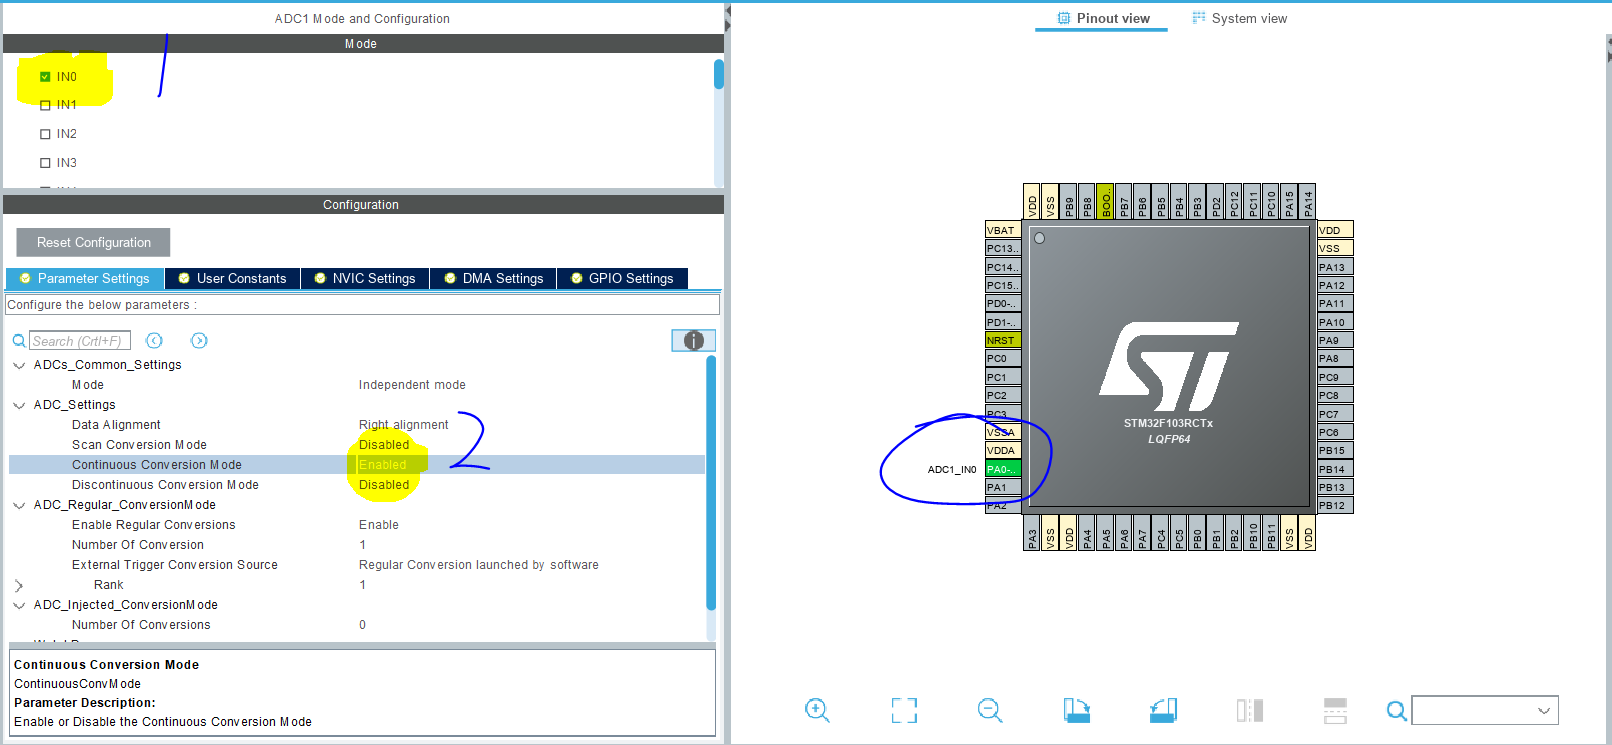
\includegraphics[width=1.0\textwidth]{adc_1.png}
	\caption{使能ADC引脚 \label{fig:scatter}}
\end{figure}

\subsection{编写业务代码-轮询方式}
\lstset{language=C}
\begin{lstlisting}
while(1){
	HAL_ADC_Start(&hadc1);//启动ADC装换
	HAL_ADC_PollForConversion(&hadc1, 50);//等待转换完成,第二个参数表示超时时间,单位ms.
	if(HAL_IS_BIT_SET(HAL_ADC_GetState(&hadc1), HAL_ADC_STATE_REG_EOC)){
		AD_Value = HAL_ADC_GetValue(&hadc1);//读取ADC转换数据,数据为12位
		printf("[\tmain]info:v=%.1fmv\r\n",AD_Value*3300.0/4096);//打印日志
	}
}
\end{lstlisting}

前面介绍了通过ADC轮询的方式采集单通道的数据。现在介绍一下通过DMA方式采集多通道的数据。

\subsection{Cube MX相关配置-DMA方式}
\subsubsection{初始化两个ADC通道}
\newpage
\begin{figure}[htbp]
	\centering
	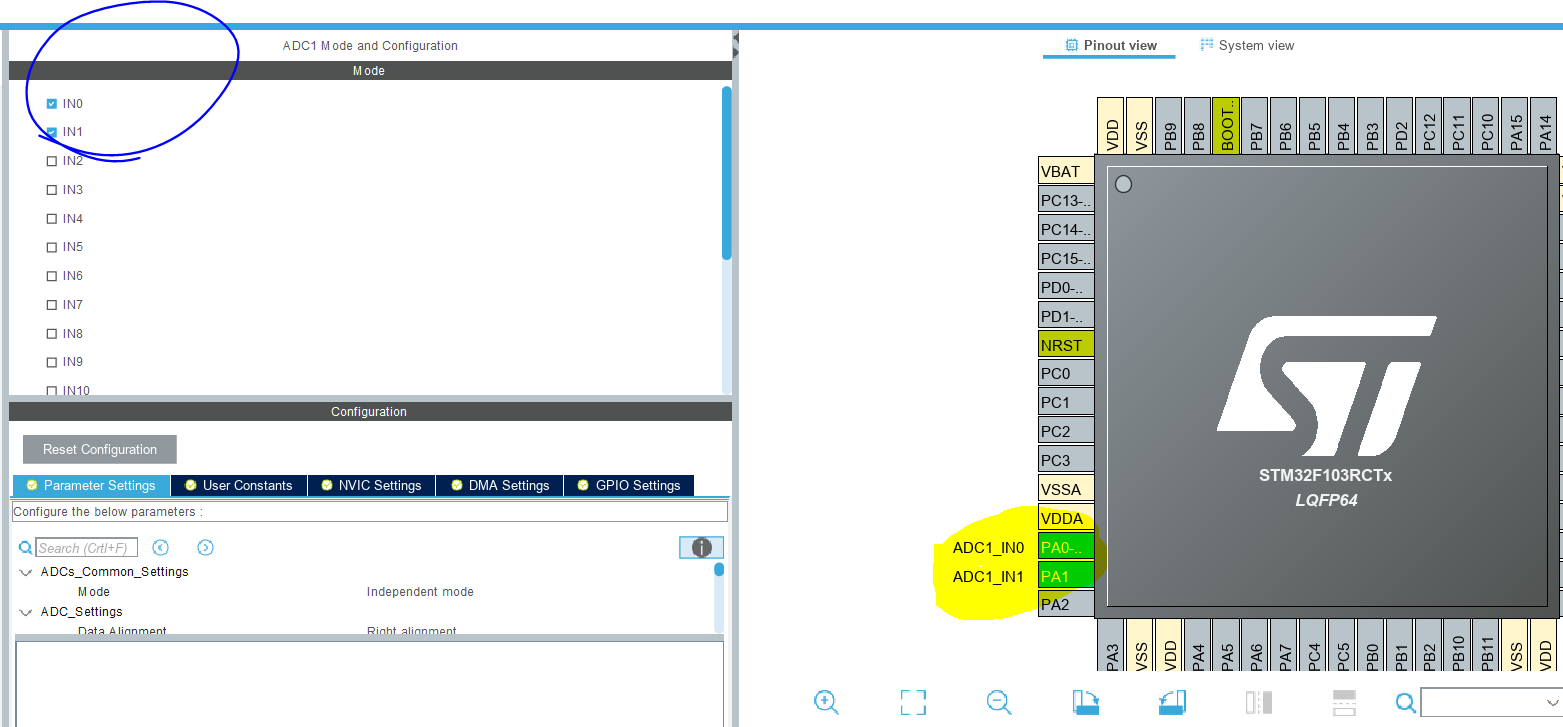
\includegraphics[width=1.0\textwidth]{adc_2.png}
	\caption{初始化两个ADC通道 \label{fig:scatter}}
\end{figure}

\subsubsection{配置相关属性}

step 1 : 使能扫描转换模式(Scan Conversion Mode),使能连续转换模式(Continuous Conversion Mode)。

step 2 : ADC规则组选择转换通道数为2(Number Of Conversion)。

step 3 : 配置Rank的输入通道。

\begin{figure}[htbp]
	\centering
	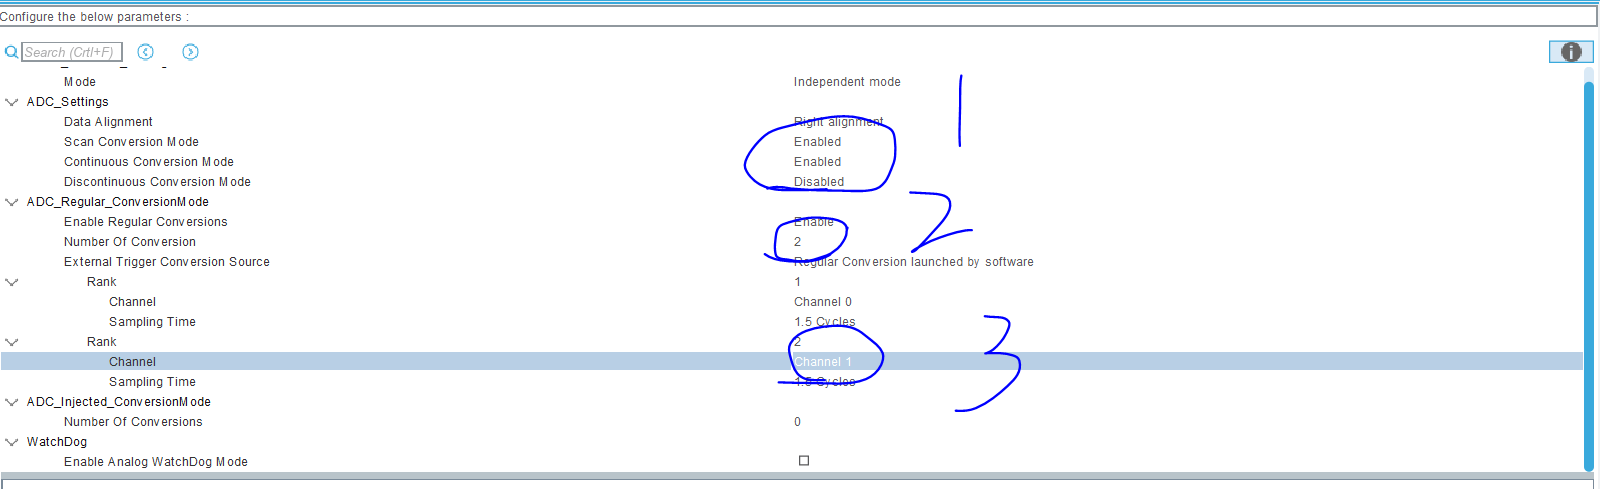
\includegraphics[width=1.0\textwidth]{adc_3.png}
	\caption{配置相关属性 \label{fig:scatter}}
\end{figure}


\subsubsection{添加DMA}
添加DMA设置,设置为连续传输模式,数据长度为字。

\begin{figure}[htbp]
	\centering
	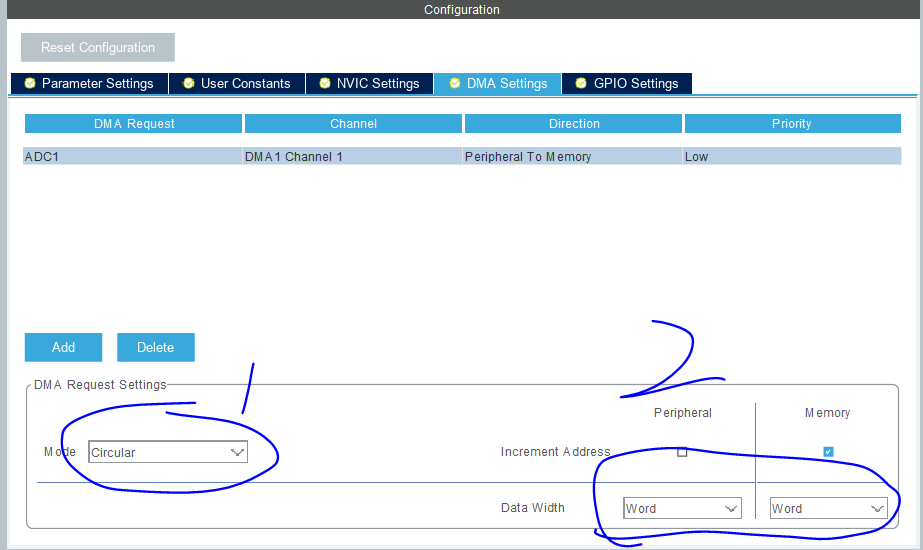
\includegraphics[width=1.0\textwidth]{adc_4.png}
	\caption{添加DMA \label{fig:scatter}}
\end{figure}

\newpage

\subsection{编写业务代码-DMA方式}

1、在main函数前面添加变量。其中ADC\_Value作为转换数据缓存数组,ad1,ad2存储PA0(转换通道0),PA1(转换通道1)的电压值。

\begin{lstlisting}
/* USER CODE BEGIN PV */
/* Private variables */
uint32_t ADC_Value[100];
uint8_t i;
uint32_t ad1,ad2;
/* USER CODE END PV */
\end{lstlisting}
2、在while(1)前面以DMA方式开启ADC装换。HAL\_ADC\_Start\_DMA()函数第二个参数为数据存储起始地址,第三个参数为DMA传输数据的长度。

\begin{lstlisting}
/* USER CODE BEGIN 2 */
HAL_ADC_Start_DMA(&hadc1, (uint32_t*)&ADC_Value, 100);
/* USER CODE END 2 */
\end{lstlisting}

由于DMA采用了连续传输的模式,ADC采集到的数据会不断传到到存储器中(此处即为数组ADC\_Value)。ADC采集的数据从ADC\_Value[0]一直存储到ADC\_Value[99],然后采集到的数据又重新存储到ADC\_Value[0],一直到ADC\_Value[99]。所以ADC\_Value数组里面的数据会不断被刷新。这个过程中是通过DMA控制的,不需要CPU参与。我们只需读取ADC\_Value里面的数据即可得到ADC采集到的数据。
其中ADC\_Value[0]为通道0(PA0)采集的数据,ADC\_Value[1]为通道1(PA1)采集的数据,ADC\_Value[2]为通道0采集的数据,如此类推。数组偶数下标的数据为通道0采集数据,数组奇数下标的数据为通道1采集数据。

在while(1)循环中添加应用程序,将采集的数据装换为电压值并输出。

\begin{lstlisting}
/* USER CODE BEGIN WHILE */
while (1){
	/* USER CODE END WHILE */
	/* USER CODE BEGIN 3 */
	HAL_Delay(500);
	for(i = 0,ad1 =0,ad2=0; i < 100;){
		ad1 += ADC_Value[i++];
		ad2 += ADC_Value[i++];
	}
	ad1 /= 50;
	ad2 /= 50;
	printf("\r\n********ADC-DMA-Example********\r\n");
	printf("[\tmain]info:AD1_value=%1.3fV\r\n", ad1*3.3f/4096);
	printf("[\tmain]info:AD2_value=%1.3fV\r\n", ad2*3.3f/4096);
}
/* USER CODE END 3 */
\end{lstlisting}
程序中将数组偶数下标数据加起来求平均值,实现均值滤波的功能,再将数据装换为电压值,即为PA0管脚的电压值。同理对数组奇数下标数据处理得到PA1管脚的电压值。

\emph{同时ADC采样也可以采用我之前描述的采用定时器对其平滑滤波!}

通常片上的ADC的精度往往达不到我们的要求,因为它的精度实在是太低了。有两个替代方案:

1、SDADC,这个是STM32F373上特有的功能,16位高速ADC,支持差分输入。掌握难度较大,我也没有很好的掌握,所以就不在此展示了。


2、ADS,就是外置ADC。在我们比赛前,我们一直调教的是ADS1256这款芯片,能做到0.01mV的精度!这类芯片只需要进行SPI通信操作,便可以获取ADC数据。


\section{DAC 数模转化}
说实话,这两年的开发中,我还没有使用过DAC的功能。但是这个功能也十分简单,配置好引脚后,编写业务代码即可。
\subsection{Cube MX相关配置}
勾选DAC中的OUT Configuration,其余配置为默认配置不需修改。
\begin{figure}[htbp]
	\centering
	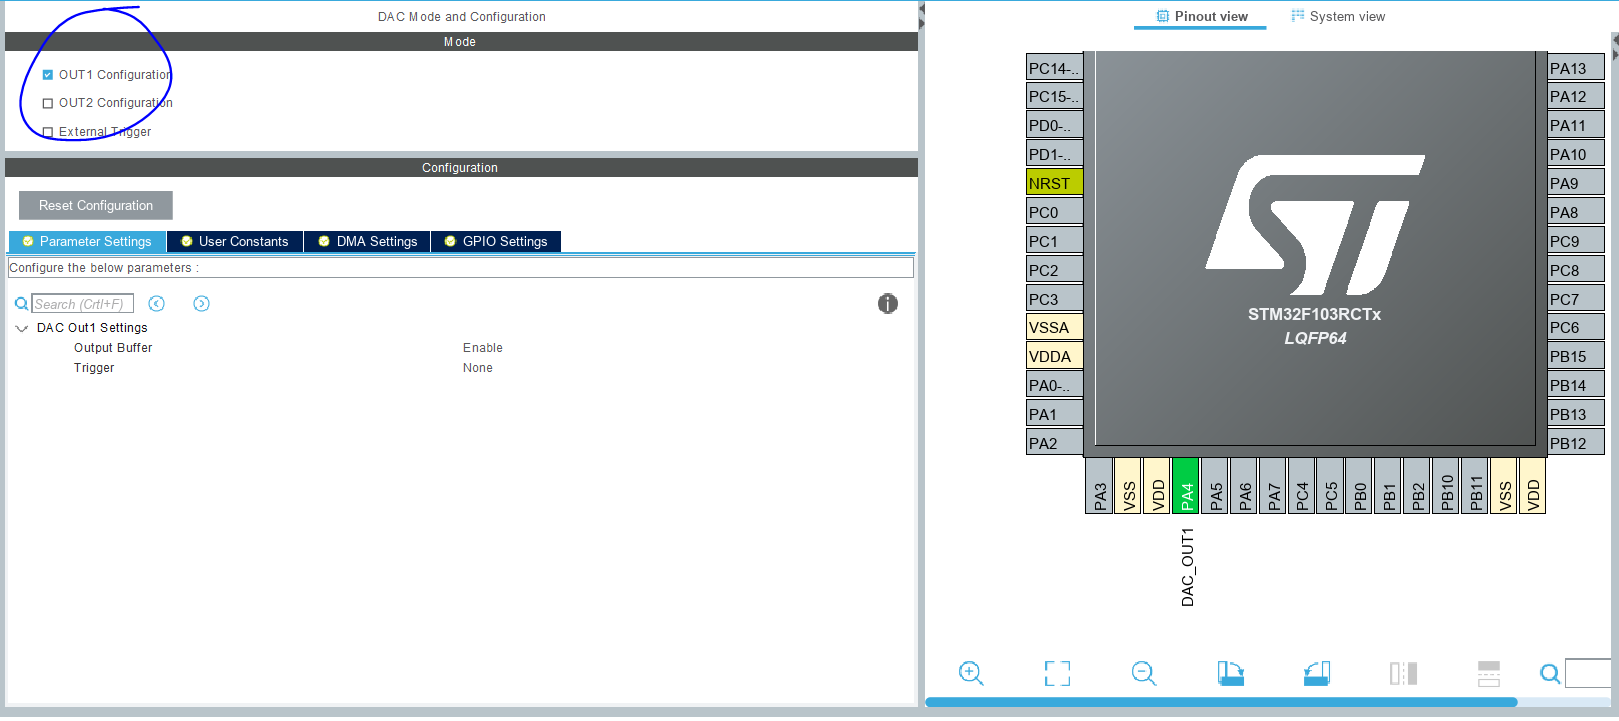
\includegraphics[width=1.0\textwidth]{dac_1.png}
	\caption{Cube MX相关配置 \label{fig:scatter}}
\end{figure}
\newpage
\subsection{编写业务代码}

\lstset{language=C}
\begin{lstlisting}
//开启DAC转换
HAL_DAC_Start(&hdac, DAC_CHANNEL_2);
// 设置DAC的大小
HAL_DAC_SetValue(&hdac, DAC_CHANNEL_2, DAC_ALIGN_12B_R, 2048); 
\end{lstlisting}
编译程序并下载到开发板。如果没有出错用万用表测管脚的电压为1.65V。

\section{I2C/SPI}
在开发中,使用到I2C/SPI的时候通常是与其他模块间的通信,例如:使用I2C与OLED通信,使用SPI与ADS1256通信。所以在此情况下,我们只需要在模块现有库函数的基础之上,做少量代码的移植即可。

\subsection{Cube MX相关配置-I2C}

直接使能I2C即可。
\begin{figure}[htbp]
	\centering
	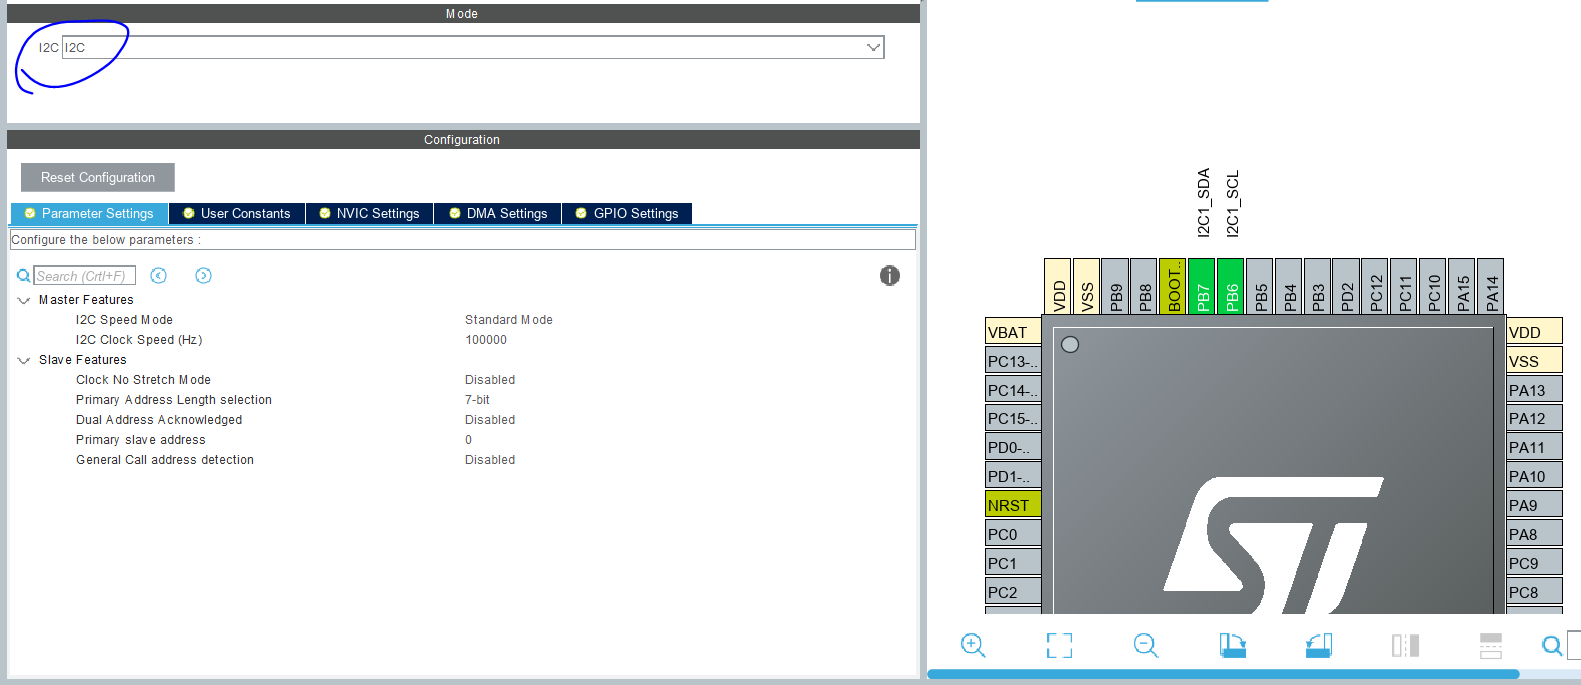
\includegraphics[width=1.0\textwidth]{i2c_1.png}
	\caption{Cube MX相关配置 \label{fig:scatter}}
\end{figure}

\newpage

\subsection{编写业务代码-I2C}

\lstset{language=C}
\begin{lstlisting}
//主机的发送
HAL_StatusTypeDef HAL_I2C_Master_Transmit(I2C_HandleTypeDef *hi2c, uint16_t DevAddress, uint8_t *pData, uint16_t Size, uint32_t Timeout);
//主机的接收
HAL_StatusTypeDef HAL_I2C_Master_Receive(I2C_HandleTypeDef *hi2c, uint16_t DevAddress, uint8_t *pData, uint16_t Size, uint32_t Timeout);
//从机的发送
HAL_StatusTypeDef HAL_I2C_Slave_Transmit(I2C_HandleTypeDef *hi2c, uint8_t *pData, uint16_t Size, uint32_t Timeout);
//从机的接收
HAL_StatusTypeDef HAL_I2C_Slave_Receive(I2C_HandleTypeDef *hi2c, uint8_t *pData, uint16_t Size, uint32_t Timeout);
\end{lstlisting}

\subsection{OLED的移植-I2C}

\subsubsection{原有库函数的代码}
\lstset{language=C}
\begin{lstlisting}
...
void I2C_Configuration(void){

	I2C_InitTypeDef  I2C_InitStructure;
	GPIO_InitTypeDef  GPIO_InitStructure; 
	
	RCC_APB1PeriphClockCmd(RCC_APB1Periph_I2C1,ENABLE);
	RCC_APB2PeriphClockCmd(RCC_APB2Periph_GPIOB,ENABLE);
	
	GPIO_InitStructure.GPIO_Pin =  GPIO_Pin_6 | GPIO_Pin_7;
	GPIO_InitStructure.GPIO_Speed = GPIO_Speed_50MHz;
	GPIO_InitStructure.GPIO_Mode = GPIO_Mode_AF_OD;
	GPIO_Init(GPIOB, &GPIO_InitStructure);
	
	I2C_DeInit(I2C1);
	I2C_InitStructure.I2C_Mode = I2C_Mode_I2C;
	I2C_InitStructure.I2C_DutyCycle = I2C_DutyCycle_2;
	I2C_InitStructure.I2C_OwnAddress1 = 0x30;
	I2C_InitStructure.I2C_Ack = I2C_Ack_Enable;
	I2C_InitStructure.I2C_AcknowledgedAddress = I2C_AcknowledgedAddress_7bit;
	I2C_InitStructure.I2C_ClockSpeed = 400000;
	
	I2C_Cmd(I2C1, ENABLE);
	I2C_Init(I2C1, &I2C_InitStructure);
}

void I2C_WriteByte(uint8_t addr,uint8_t data){

	while(I2C_GetFlagStatus(I2C1, I2C_FLAG_BUSY));
	
	I2C_GenerateSTART(I2C1, ENABLE);
	while(!I2C_CheckEvent(I2C1, I2C_EVENT_MASTER_MODE_SELECT));
	
	I2C_Send7bitAddress(I2C1, OLED_ADDRESS, I2C_Direction_Transmitter);
	while(!I2C_CheckEvent(I2C1, I2C_EVENT_MASTER_TRANSMITTER_MODE_SELECTED));
	
	I2C_SendData(I2C1, addr);
	while (!I2C_CheckEvent(I2C1, I2C_EVENT_MASTER_BYTE_TRANSMITTED));
	
	I2C_SendData(I2C1, data);
	while (!I2C_CheckEvent(I2C1, I2C_EVENT_MASTER_BYTE_TRANSMITTED));
	
	I2C_GenerateSTOP(I2C1, ENABLE);
}

void WriteCmd(unsigned char I2C_Command){
	I2C_WriteByte(0x00, I2C_Command);
}

void WriteDat(unsigned char I2C_Data){
	I2C_WriteByte(0x40, I2C_Data);
}

void OLED_Init(void){
	DelayMs(100);

...
\end{lstlisting}

\subsubsection{移植代码分析}

I2C\_Configuration 其实就是I2C的初始化函数,Cube MX 会帮我们生成,所以直接删除

I2C\_WriteByte 被接下来的两个函数依赖,但是HAL中有相应的函数,所以直接删除

WriteCmd和WriteDat改写成HAL库的方式

DelayMs改为HAL库中的函数

\subsubsection{移植后的代码}
\begin{lstlisting}
...
#include "i2c.h"

void WriteCmd(unsigned char I2C_Command){
	HAL_I2C_Mem_Write(&hi2c1,OLED_ADDRESS,0x00,I2C_MEMADD_SIZE_8BIT,&I2C_Command,1,100);
}

void WriteDat(unsigned char I2C_Data){
	HAL_I2C_Mem_Write(&hi2c1,OLED_ADDRESS,0x40,I2C_MEMADD_SIZE_8BIT,&I2C_Data,1,100);
}

void OLED_Init(void){
	HAL_Delay(100);
...
\end{lstlisting}

\subsection{Cube MX相关配置-SPI}

使能SPI后,但是需要根据设备的不同做分频处理。

\begin{figure}[htbp]
	\centering
	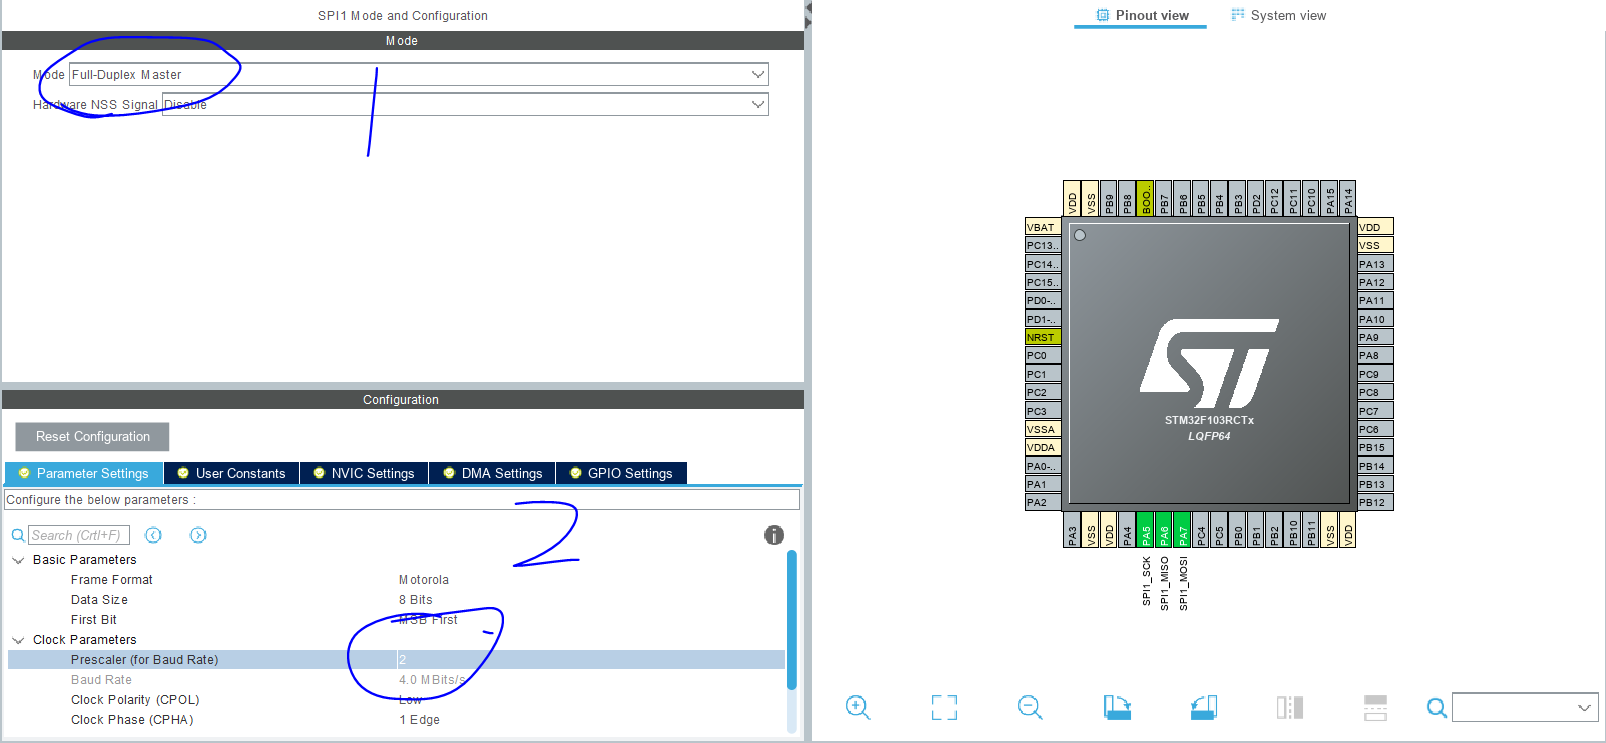
\includegraphics[width=1.0\textwidth]{spi_1.png}
	\caption{Cube MX相关配置 \label{fig:scatter}}
\end{figure}

\newpage
\subsection{编写业务代码-SPI}

\lstset{language=C}
\begin{lstlisting}
//SPI的发送
HAL_StatusTypeDef HAL_SPI_Transmit(SPI_HandleTypeDef *hspi, uint8_t *pData, uint16_t Size, uint32_t Timeout);
//SPI的接收
HAL_StatusTypeDef HAL_SPI_Receive(SPI_HandleTypeDef *hspi, uint8_t *pData, uint16_t Size, uint32_t Timeout);
//SPI的发送和接收
HAL_StatusTypeDef HAL_SPI_TransmitReceive(SPI_HandleTypeDef *hspi, uint8_t *pTxData, uint8_t *pRxData, uint16_t Size,
uint32_t Timeout);
\end{lstlisting}

\subsection{ADS1256的移植-SPI}

SPI的移植比I2C的移植要难并且复杂很多,基本上所有的函数都需要做大大小小的改动,建议大家尽量不要自己移植,最好是在网上找到相关的资源。


\section{FLASH}

FLASH的操作,不需要使用Cube MX做任何的配置,只需要做编程操作即可。

\subsection{相关定义}
\lstset{language=C}
\begin{lstlisting}
#define BaseAddress  ((uint32_t)0x080E0000) // 操作FLAH基地址
//需根据自己单片机的型号进行修改

uint32_t paper_table[100] = {0} ;//需要写入FLAH中的第一张表
uint32_t pwm_table[100] = {0};//需要写入FLAH中的第二张表
uint32_t length_table = 0;
\end{lstlisting}

\subsection{FLAH的写入}

\emph{注意:我接下来提供的例程是来自STM32F407,不同板子间的FLASH\_EraseInitTypeDef可能不同。}

\lstset{language=C}
\begin{lstlisting}
HAL_FLASH_Unlock();

FLASH_EraseInitTypeDef f;

f.TypeErase = FLASH_TYPEERASE_SECTORS; 
//F103中为FLASH_TYPEERASE_PAGES,即页擦除
f.Sector = FLASH_SECTOR_11;
//F103中为  f.PageAddress = BaseAddress 即开始操作的地址为BaseAddress
f.NbSectors = 1;
//F103中为  f.NbPages = x,即擦除x页


//设置PageError
uint32_t PageError = 0;
//调用擦除函数
HAL_FLASHEx_Erase(&f, &PageError);
//对FLASH烧写
for(int i = 0; i < 100; i++) {
	HAL_FLASH_Program(TYPEPROGRAM_WORD, (BaseAddress +  4 * i),  paper_table[i]);
}
for(int i = 0; i < 100; i++) {
	HAL_FLASH_Program(TYPEPROGRAM_WORD, (BaseAddress + 400 +  4 * i),  pwm_table[i]);
}
//锁住FLASH
HAL_FLASH_Lock();
\end{lstlisting}

\subsection{FLAH的读取}
FLAH的读取十分简单,只需要读取相应地址上的值即可。

\begin{lstlisting}
for(int i = 0; i < 100; i++) {
	paper_table[i] =  *(__IO uint32_t*) (BaseAddress +  4 * i);
}

for(int i = 0; i < 100; i++) {
	pwm_table[i] =  *(__IO uint32_t*) (BaseAddress + 400 + 4 * i);
}
while(paper_table[length_table] != 0) {
	length_table++;
}
\end{lstlisting}

\section{算法-排序}

这两个模板,是我用了很久的,通过长时间的测试,我向你保证它是绝对的可靠!



\subsection{快速排序}

\lstset{language=C}
\begin{lstlisting}
void quick_sort(int q[], int l, int r){
	if (l >= r) return;
	
	int i = l - 1, j = r + 1, x = q[l];
	while (i < j){
	do i ++ ; while (q[i] < x);
	do j -- ; while (q[j] > x);
	if (i < j) {
		q[i] = q[i]^q[j];
		q[j] = q[i]^q[j];
		q[i] = q[i]^q[j];
	}
	else break;
	}
	quick_sort(q, l, j), quick_sort(q, j + 1, r);
}
\end{lstlisting}

\subsection{归并排序}

\lstset{language=C}
\begin{lstlisting}
void merge_sort(int q[], int l, int r){
	if (l >= r) return;
	
	int mid = l + r >> 1;
	merge_sort(q, l, mid);
	merge_sort(q, mid + 1, r);
	
	int k = 0, i = l, j = mid + 1;
	while (i <= mid && j <= r)
	if (q[i] < q[j]) tmp[k ++ ] = q[i ++ ];
	else tmp[k ++ ] = q[j ++ ];
	
	while (i <= mid) tmp[k ++ ] = q[i ++ ];
	while (j <= r) tmp[k ++ ] = q[j ++ ];
	
	for (i = l, j = 0; i <= r; i ++, j ++ ) q[i] = tmp[j];
}
\end{lstlisting}
\section{算法-MPPT}

在做最大功率点追踪,这个算法是十分重要的。我在这里分享一下我是怎么对其优化的,首先我写了一个能实现功能的最基础的版本。

\subsection{基础版本}

\lstset{language=C}
\begin{lstlisting}
#include "mppt.h"
#include "main.h"
#include "usart.h"

//上一次的功率
double l_power = 0.0 ;
//功率上升或下降
int updown = 0;
//步长
int MPPT_STEP = 160;

/* 扰动法计算
*
*/
int mppt_po(double u, double i, int pwm) {

	double power = (u * i) < 0 ? 0 : u * i ;
	
	printf("[Info]mppt_po:当前电流:%f,当前电压:%f,当前功率:%f\r\n", i, u, power);
	
	if(power < l_power || power == 0) {
		updown ^= 1;
		printf("[Info]mppt_po:当前功率:%f,小于此前功率:%f\r\n", power, l_power);
	}
	
	if(updown) {
		printf("[Info]mppt_po:PWM:%d调节为:%d\r\n", pwm, pwm + MPPT_STEP);
		pwm += MPPT_STEP;
	
	}
	else {
		printf("[Info]mppt_po:PWM:%d调节为:%d\r\n", pwm, pwm - MPPT_STEP);
		pwm -= MPPT_STEP;
	}
	
	printf("[Info]mppt_po:该次调节结束\r\n");
	
	pwm = pwm < 0 ? 0 : (pwm >= 1599 ? 1599 : pwm);
	
	l_power = power;
	
	return pwm;
}

\end{lstlisting}

\subsection{算法的不足与解决方案}

1、这个算法一直在调节,这很有可能造成能量的损耗。 解决方案:采用标志位,判断是否稳定。

2、这个算法步长不变,从头到尾固定步长。如果步长太长不精细,如果步长太短整体调节较慢。解决方案:采用可变步长。

3、使用三目运算符取代大量的if-else

4、Log信息采用条件编译的方法(  很早之前写的,没能采用串口的终极解决方案,有点遗憾) 

5、抽离变量,写出结构体,配以初始化函数。

\subsection{最终版本}

\lstset{language=C}
\begin{lstlisting}
/**
  * @file :mppt.c
  *
  * @brief: MPPT 最大功率点追踪
  *
  * @auther : Reyunn
  *
  */
#include "mppt.h"
#include "main.h"
#include "usart.h"

extern void quick_sort(int q[], int l, int r);

typedef struct {
	double l_power;//上一次的功率
	uint8_t updown;//功率上升或下降
	int max_step;//步长
	int min_step;//步长
	int pwm_max ; //pwm最大值
	int pwm_min ; //pwm最小值
	uint8_t count; //计算微调次数
	uint8_t state; //状态
	uint8_t time; //改变方向次数
	int l_pwm[10];
} MPPT;

MPPT mppt;

/**
* @brief mppt 初始化
* @param l_power : 上次测量功率
* @param updown : 上升或下降
* @param min_step :最小步长
* @param max_step :最大步长
* @param pwm_max : pwm最大值
* @param pwm_min : pwm最小值
* @retval None
*/
void mppt_init(double l_power, uint8_t updown, int min_step, int max_step, int pwm_max, int pwm_min) {
	mppt.l_power = l_power;
	mppt.updown = updown;
	mppt.max_step =  max_step;
	mppt.min_step =  min_step;
	mppt.pwm_max = pwm_max;
	mppt.pwm_min = pwm_min;
	mppt.count = 0;
	mppt.state = 1;
	mppt.time = 0;
}

/**
* @brief 扰动法计算
* @param u : 当前电压值
* @param i :当前电流值
* @param pwm : 当前pwm值
* @retval 计算后的pwm值
*/
int mppt_po(double u, double i, int pwm) {

	double power = (u * i) < 0 ? 0 : u * i ;
	
	if(mppt.state) {
	
#if Log
	printf("[info]mppt_po:当前电流:%f,当前电压:%f,当前功率%f\r\n", i, u, power);
#endif
	
	if(power < mppt.l_power  || pwm == mppt.pwm_max || pwm == mppt.pwm_min) {
		mppt.updown ^= 1;
		mppt.time ++;
		
		if(mppt.time > 5 && power < mppt.l_power )  mppt.l_pwm[mppt.count++] = pwm;
#if Log
		printf("[info]mppt_po:当前功率:%f,小于此前功率%f\r\n", power, mppt.l_power);
#endif
	}
	pwm = (mppt.updown == 1) ? ((mppt.count > 0) ? pwm + mppt.min_step : pwm + mppt.max_step) : ( (mppt.count > 0 ) ? pwm -  mppt.min_step : pwm - mppt.max_step);
	
	pwm = (pwm < mppt.pwm_min ) ? mppt.pwm_min : ( (pwm >= mppt.pwm_max) ? mppt.pwm_max : pwm);
	
	mppt.l_power = power;	
	
	if(mppt.count == 10) {
		mppt.state = 0;
		quick_sort(mppt.l_pwm, 0, 9);
		return ( mppt.l_pwm[5] + mppt.l_pwm[4] + mppt.l_pwm[3] + mppt.l_pwm[6] ) / 4;
	}
	return pwm;
	} else {
	
		if( power - mppt.l_power > 1000 || power - mppt.l_power < -1000 ){
		mppt.count = 0;
		mppt.state = 1;
		mppt.time = 0;
#if Log
		printf("[info]mppt.c:进入调整模式\r\n");
#endif
	}
	return pwm;
	}

}


\end{lstlisting}


\section{后记}

这个STM32部分的内容,到目前(  2019年8月26日 ) 为止共有两次改动。

v1.0.x : 第一次版本。

v1.1.x : 在第一次的基础上,有以下改动:

1、规范目录结构。

2、增多串口通信、ADC内容。

3、增加I2C/SPI及FLASH的内容。

4、删除Astyle等内容。

同时这个部分的内容,也是作为信息学院2019年暑假集训的讲义,期间大家相互学习。在和电子科技协会全体会员的一起努力下,我们共同录制了一套CubeMX + MDK5 + HAL库 + 库函数一站式学习STM32的学习视频。
	
\begin{figure}[htbp]
	\centering
	
\includegraphics[width=0.4\textwidth]{hou.png}
	\caption{ STM32系列视频 \label{fig:scatter}}
\end{figure}

如果你想仅仅学习HAL库就完全掌握STM32那是不可能的,在此之前你必须对寄存器、库函数这两种开发方式有一定的了解。

但是如果学习到此你就认为你完全掌握了STM32那也是不可能的,往后还有DSP、FreeRTOS等需要你学习。

\chapter{四天三夜}

2019年8月7号开始,为期四天三夜的电子设计大赛拉开了序幕,这次的比赛整个经历对我来说是一笔大的财富。这次的比赛总的来说没走什么弯路,第一天将硬件搭出来了,第二天做实验找规律,第三天写程序,第四天测试写报告。

\section{第一天 - 2019.08.07}
今早7点30分,大赛主委会公布了本次大赛的题目。本科组的题目:A 电动小车动态无线充电系统、B	巡线机器人、C	线路负载及故障检测装置、D	简易电路特性测试仪、E	基于互联网的信号传输系统、F	纸张计数显示装置、G	双路语音同传的无线收发系统、H	模拟电磁曲射炮。对于一直在做电源的我们来说,选择有两个:1、A 电动小车动态无线充电系统 2、H	模拟电磁曲射炮 。 但是A题必须使用TI的处理器,H题则和控制类联系十分紧密,所以这两道题对我们来说都很难做。考虑多方面的因素以及老师的建议,我们最终选择了F题纸张计数显示装置。

\begin{figure}[htbp]
	\centering
	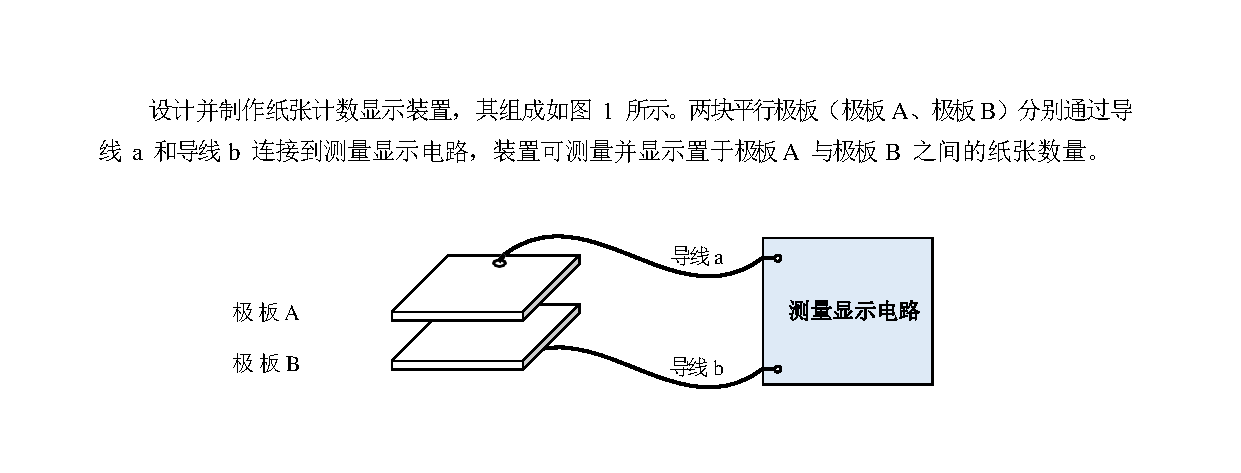
\includegraphics[width=1.0\textwidth]{F.pdf}
	\caption{F题截选 \label{fig:scatter}}
\end{figure}


这是一道仪器测量类的题目,简单的来说就是 测纸张 == 测两极板间的电容。但是这道题的难点并不在于测电容,因为测量电容的方法有很多:使用FDC2214芯片直接通过通信读取两极板间的电容、利用LC谐振测量... 这道题真正的难点在于将测量的电容值转化为纸张数。

刚开始我们也不知道电容与纸张数之间的关系到底是什么,所以今天我们的首要任务就是将硬件搭起来,通过实验找去两者之间的关系。我们的硬件方案选择的是利用NE555的震荡将电容值转化为PWM的频率,再将PWM频率与纸张数对应起来。


\section{第二天 - 2019.08.08}

比赛的第二天,有了昨天的硬件基础,我们今天的任务就是疯狂的做实验了。放纸-> 测量 -> 放纸 -> 测量 ...同时我们进行的还有完善硬件结构,使其更牢固。用什么东西压极板是个大问题,尝试过用砖头、水瓶、沙袋、但是效果都不近人意,最后我们还是在淘宝上找了家大理石加工店,给我们加工了两块4cm*4cm*4cm的石块。在使用不同压重物的情况下,测量出以下数据:可以得出两个结论:1、在纸张数较小的情况下呈线性关系 2、纸张数越多频率变化越小。

\begin{figure}[htbp]
	\centering
	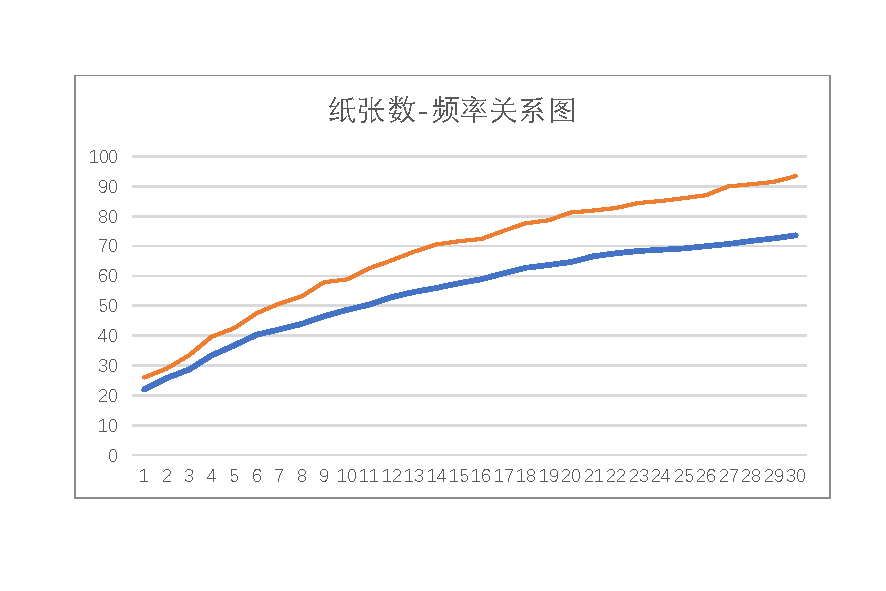
\includegraphics[width=1.0\textwidth]{data.pdf}
	\caption{纸张数-频率关系 \label{fig:scatter}}
\end{figure}

\section{第三天 - 2019.08.09}
比赛的第三天,就是写程序了。

最重要的问题就是如何拟合?首先我的想法是采用多项式拟合,我知道apache有个开源的math3有很多的拟合工具,但是他是采用Java开发的,所以我们想法是“移植”。但是在老师的分析下,因为这个曲线在任意两点间还是接近线性的存在,并且编程简单。其次,如何采样的更准?滤波!What's more ? 标定数据的处理!保存Flash、修改、删除。这些所有的细节在stm32部分我都会做详细的描述。

这个晚上的3点钟,修改完最后一个Bug。程序定型,不再修改。


\section{第四天 - 2019.08.10}
比赛进行到现在,硬件、软件都没什么好修改的了,需要练习的就是放纸的手法了。也做了很多次的模拟,测试我们系统的可靠性。最好的测试结果就是1-30张纸没有错误,30-41张纸存在2个错误。

比赛进行到今天我的状态就是:目光呆滞,两眼无神。4天时间没刷过牙、没洗过脸、没洗过澡...

\begin{figure}[htbp]
	\centering
	
\includegraphics[width=0.6\textwidth]{me4.jpg}
	\caption{电赛第四天早上 \label{fig:scatter}}
\end{figure}

下午在测试完所有功能后,进行封箱的操作

\begin{figure}[htbp]
	\centering
	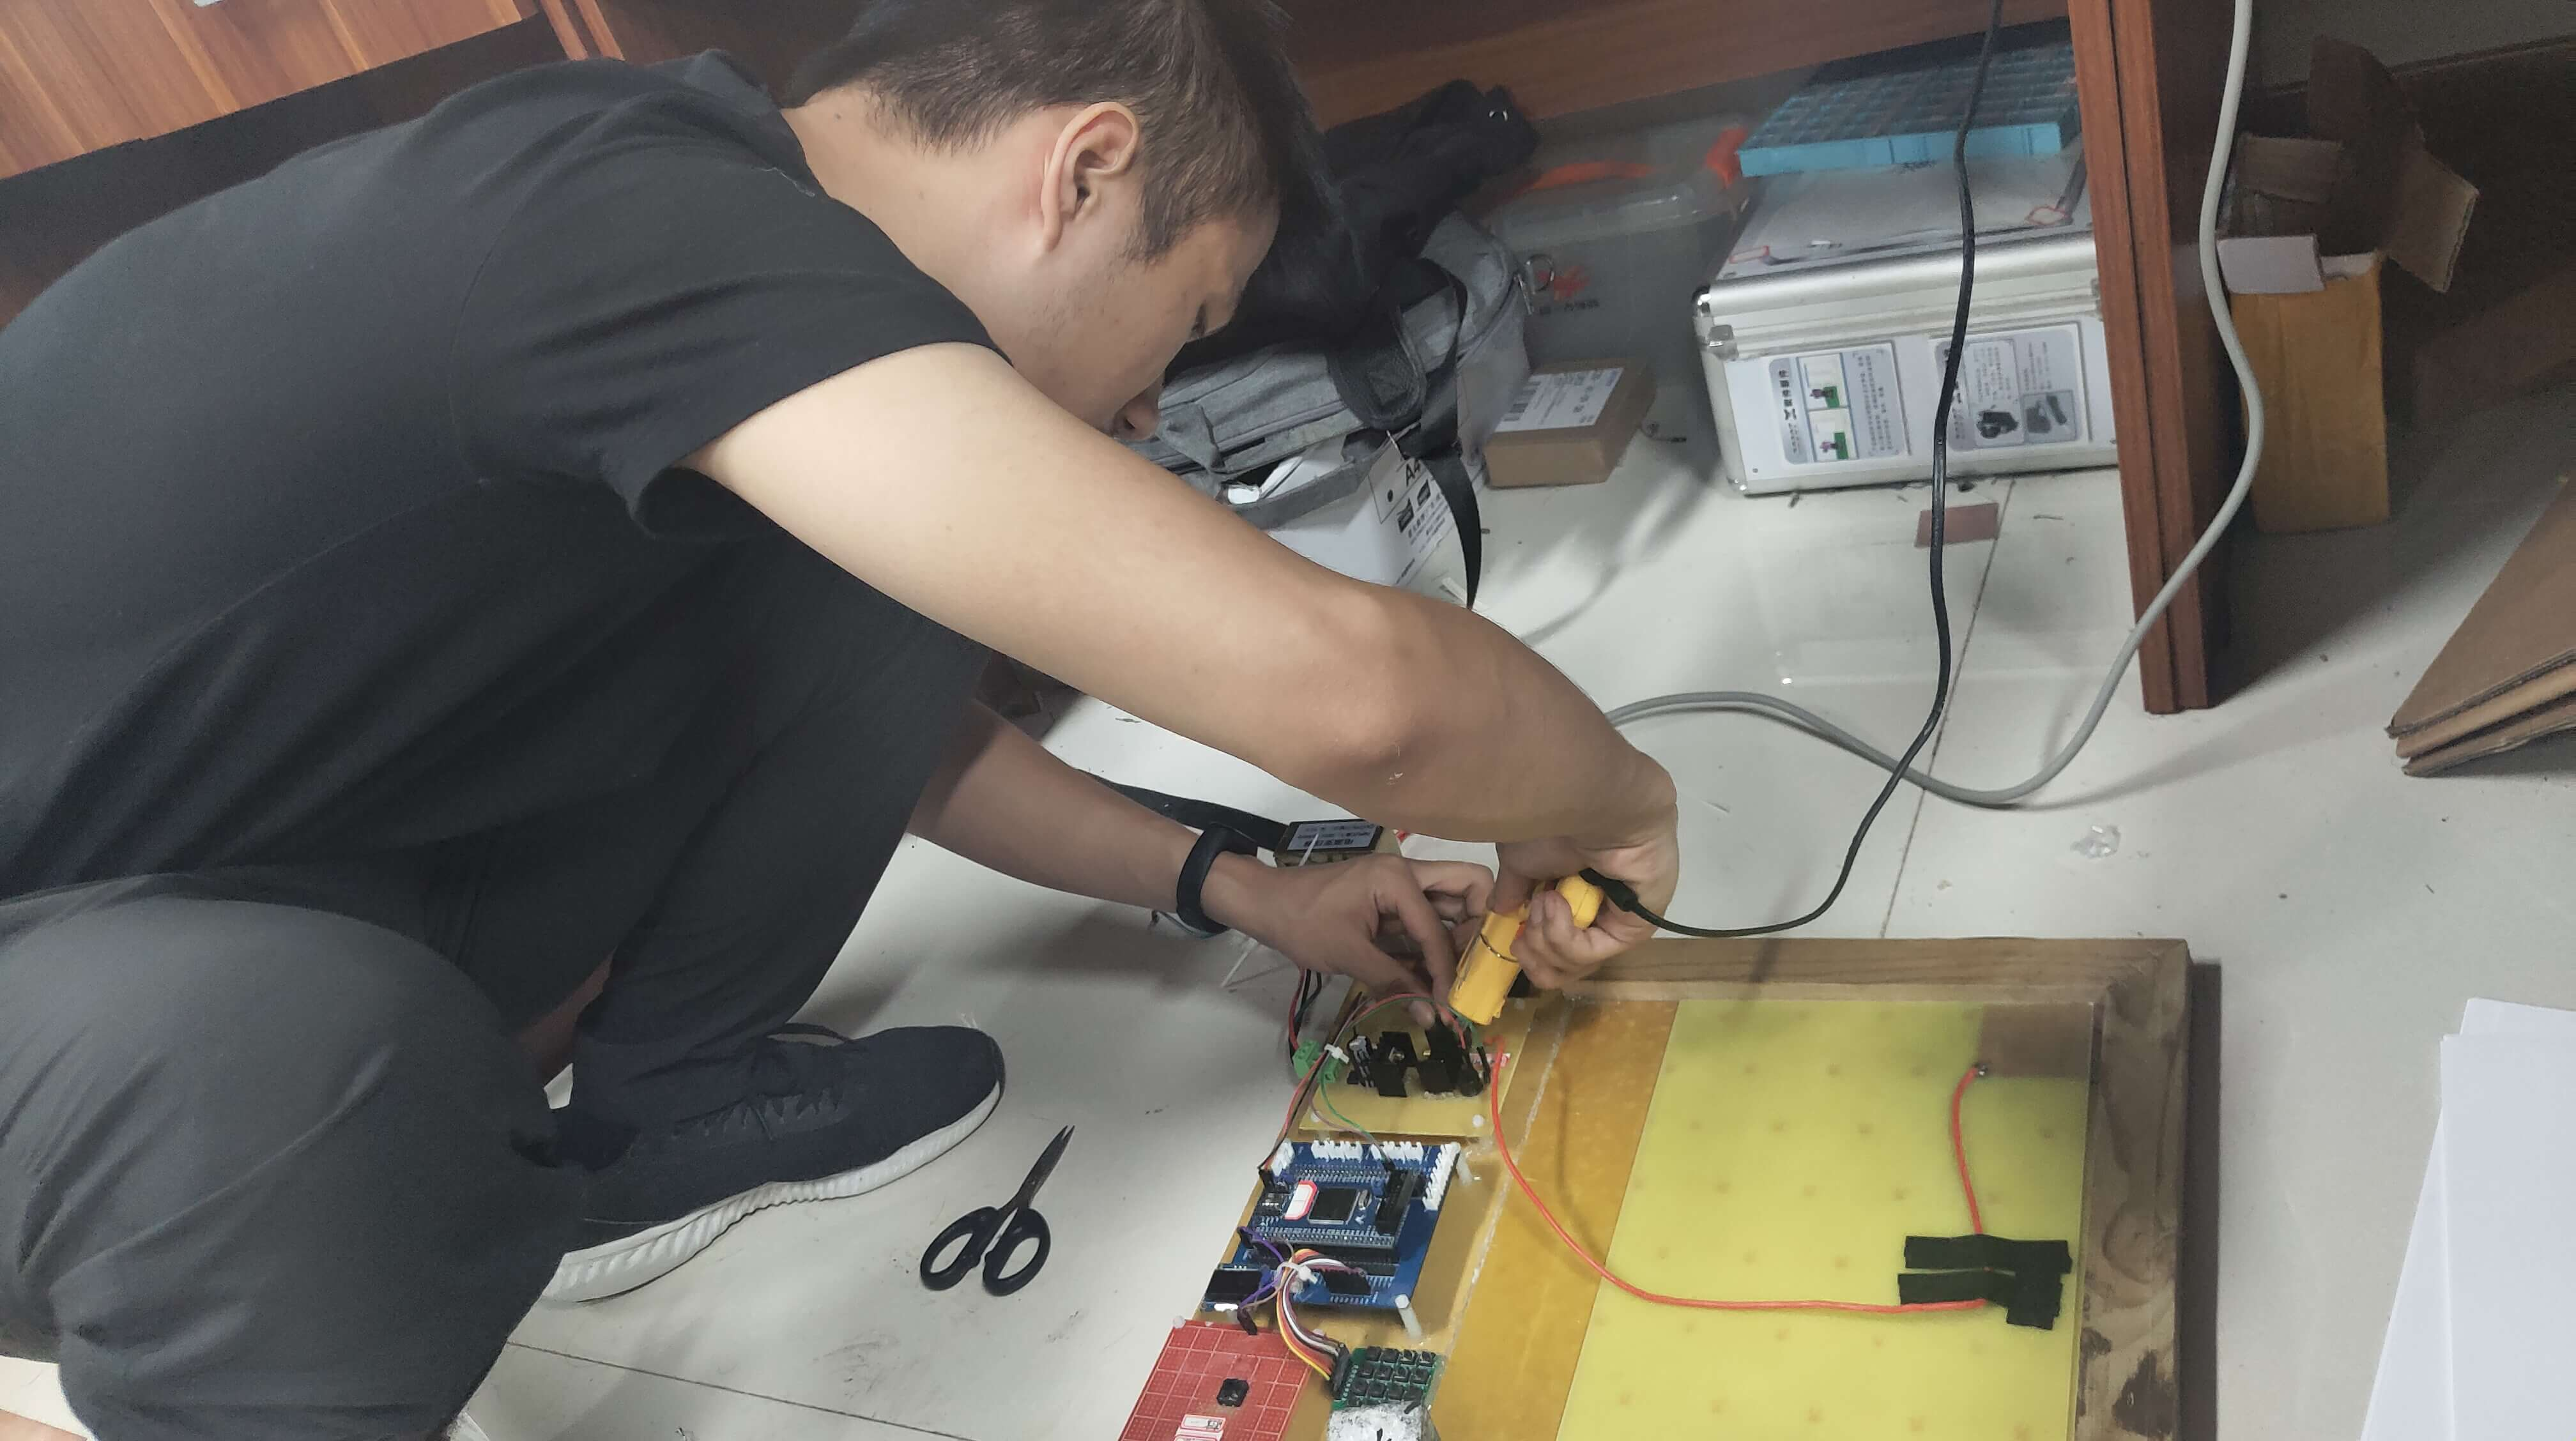
\includegraphics[width=0.8\textwidth]{me5.jpg}
	\caption{涂劲豪在封箱 \label{fig:scatter}}
\end{figure}

修改报告到焦头烂额的队友,及小帮手
\begin{figure}[htbp]
	\centering
	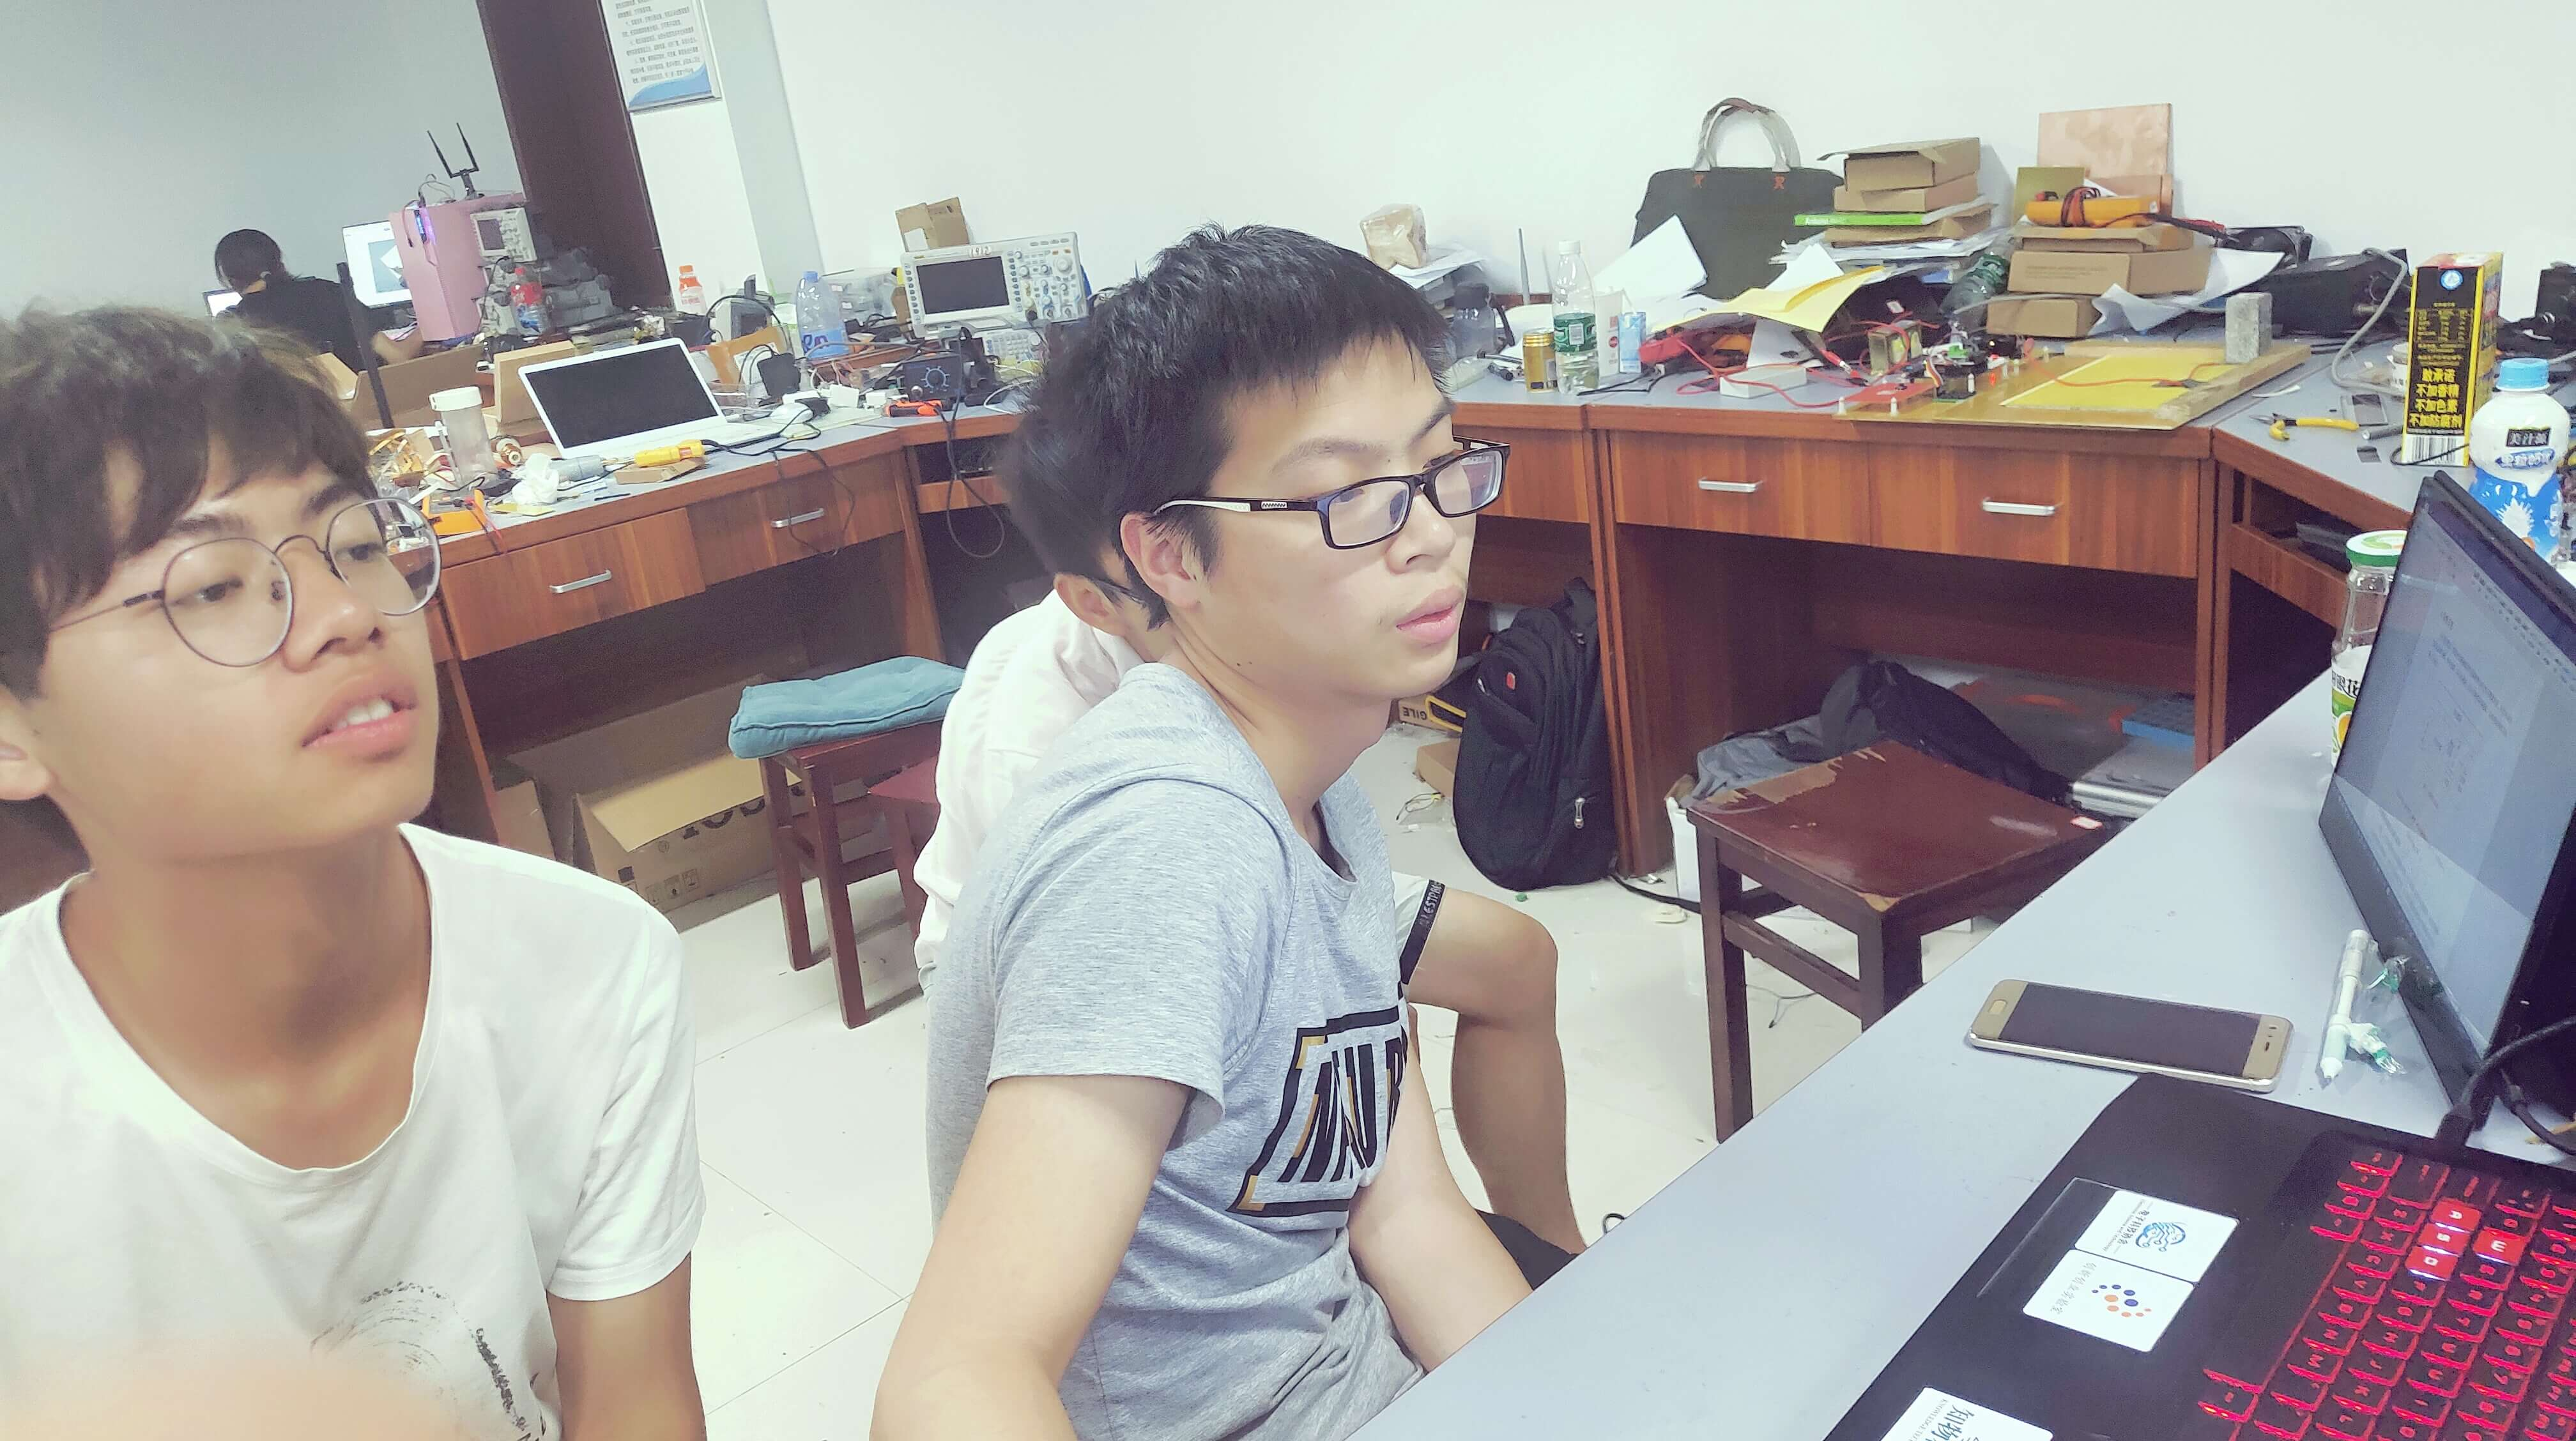
\includegraphics[width=1.0\textwidth]{me7.jpg}
	\caption{陈同凯在修改报告 \label{fig:scatter}}
\end{figure}


作品封箱前的照片

\begin{figure}[htbp]
	\centering
	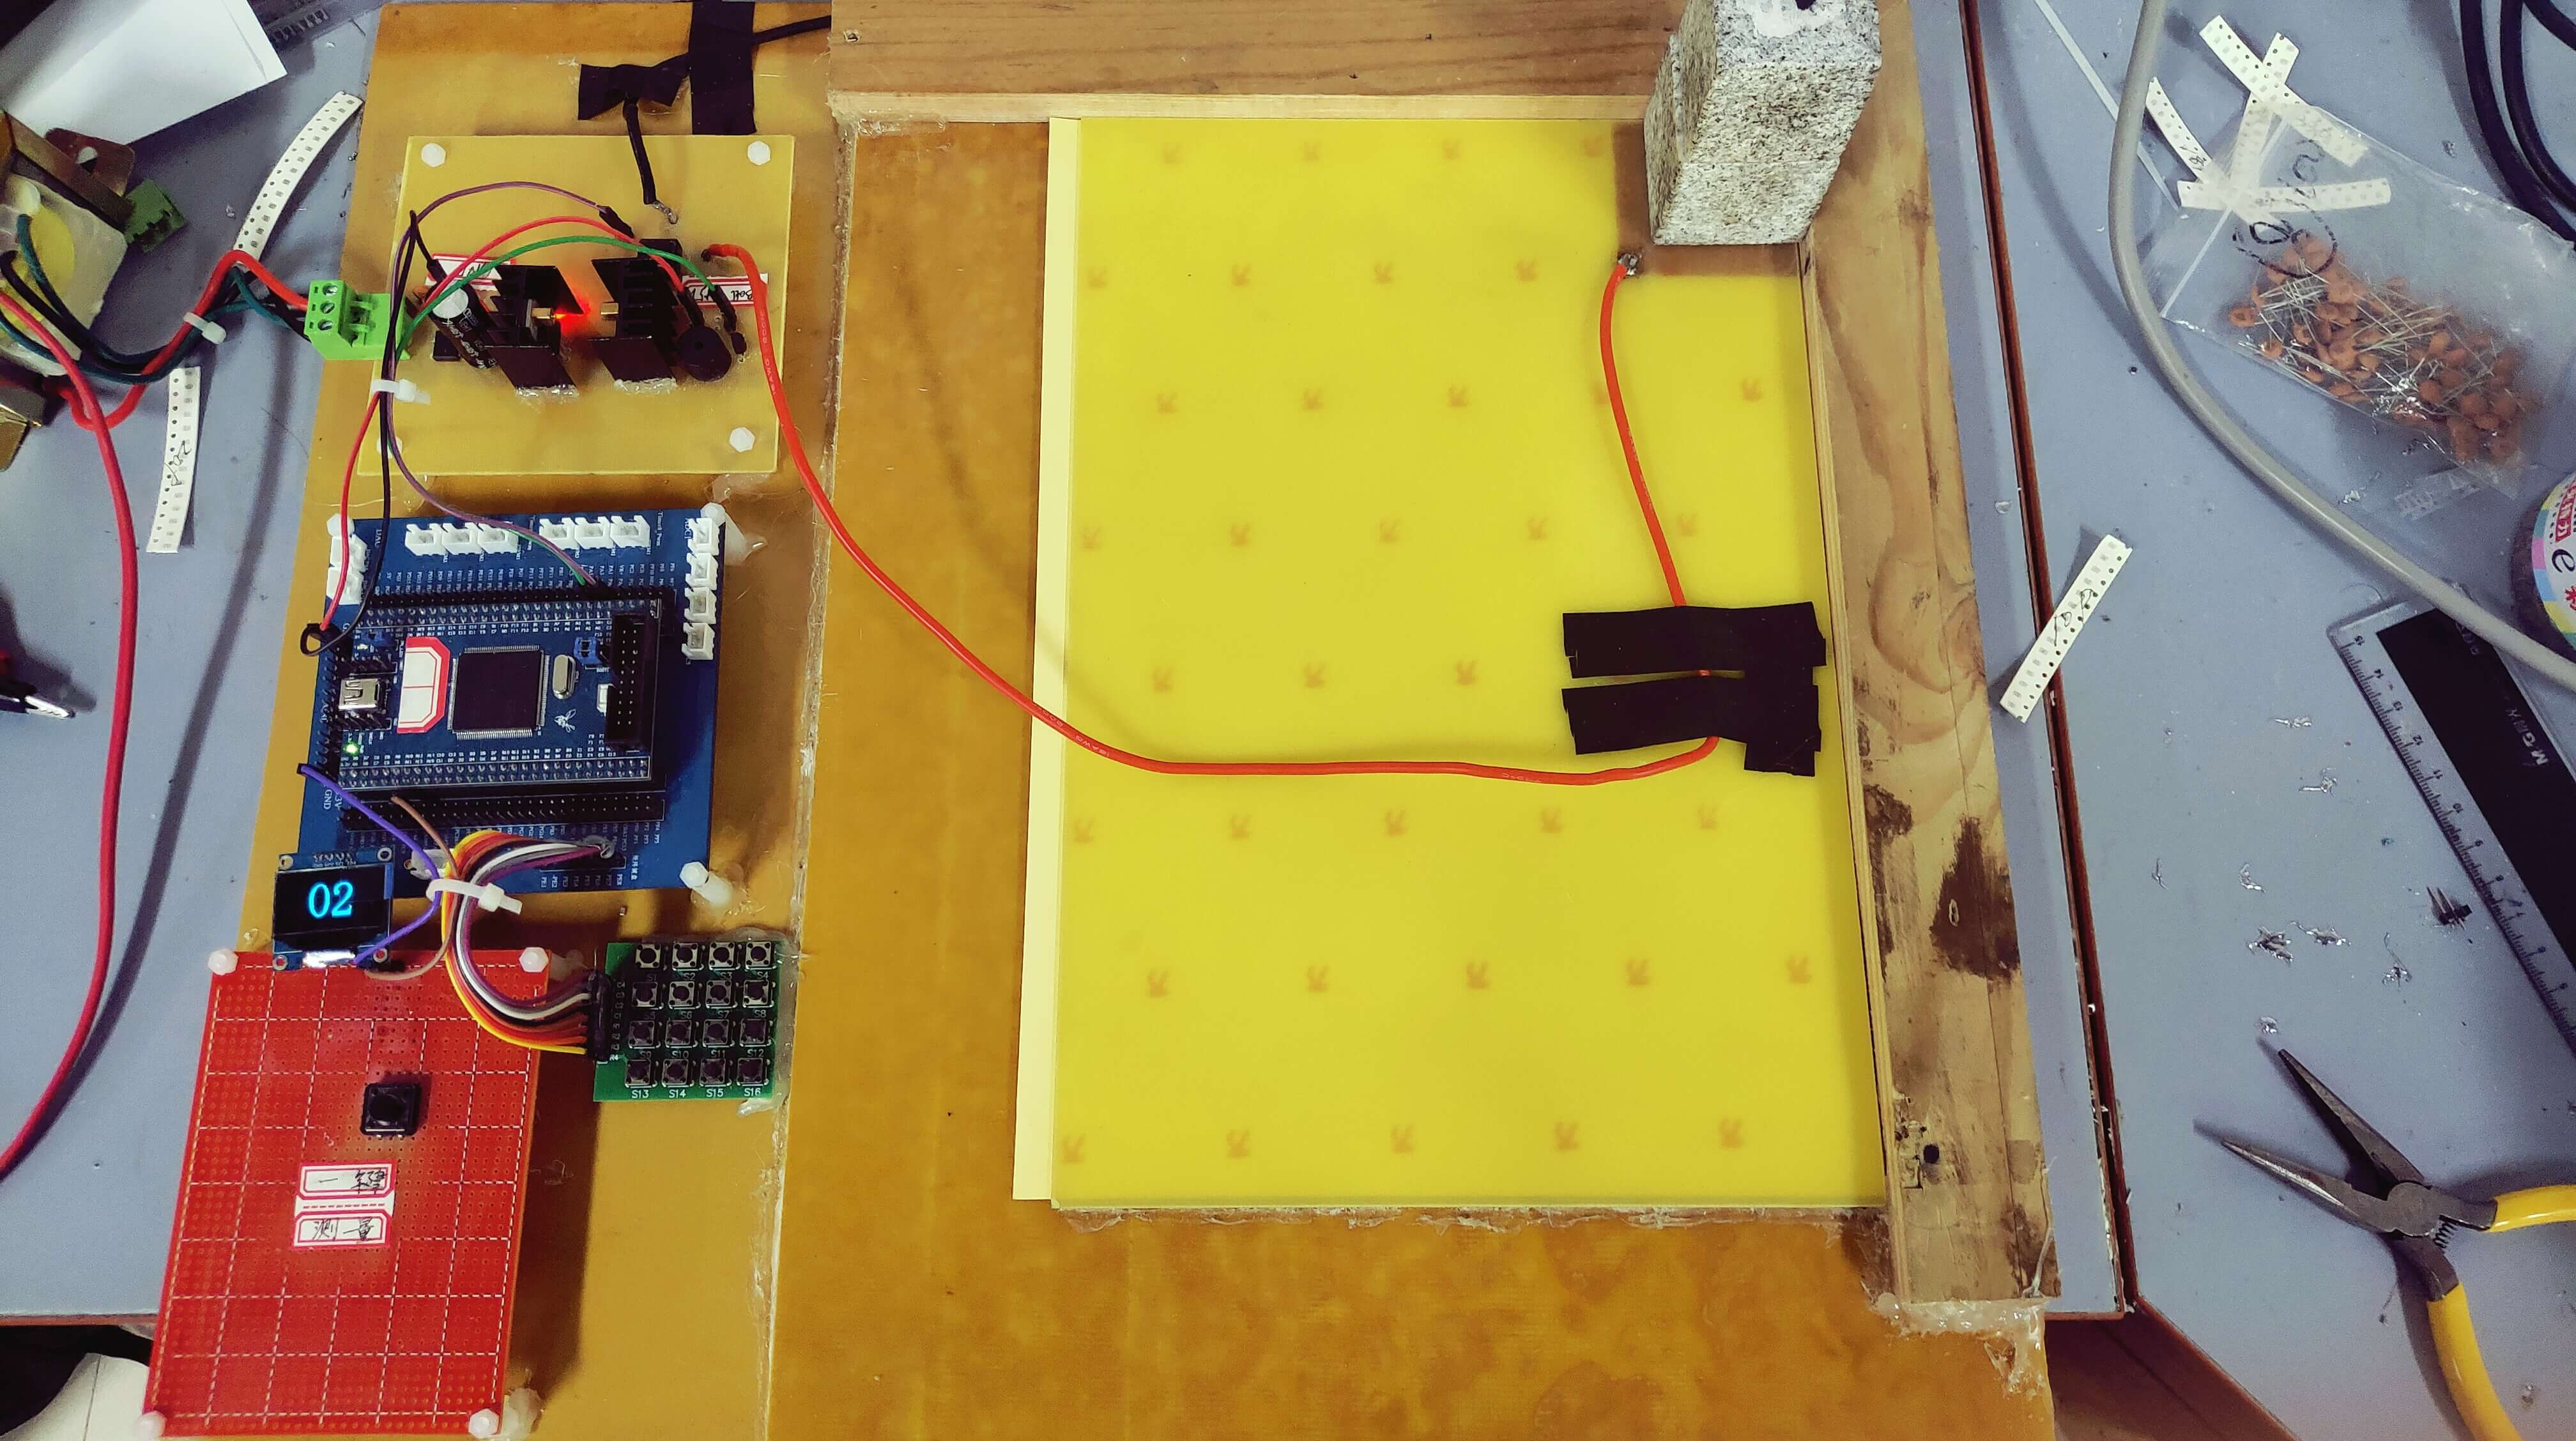
\includegraphics[width=1.0\textwidth]{me6.jpg}
	\caption{最后的成品 \label{fig:scatter}}
\end{figure}

晚上23:41将作品送至武汉大学,4天3夜结束
\begin{figure}[htbp]
	\centering
	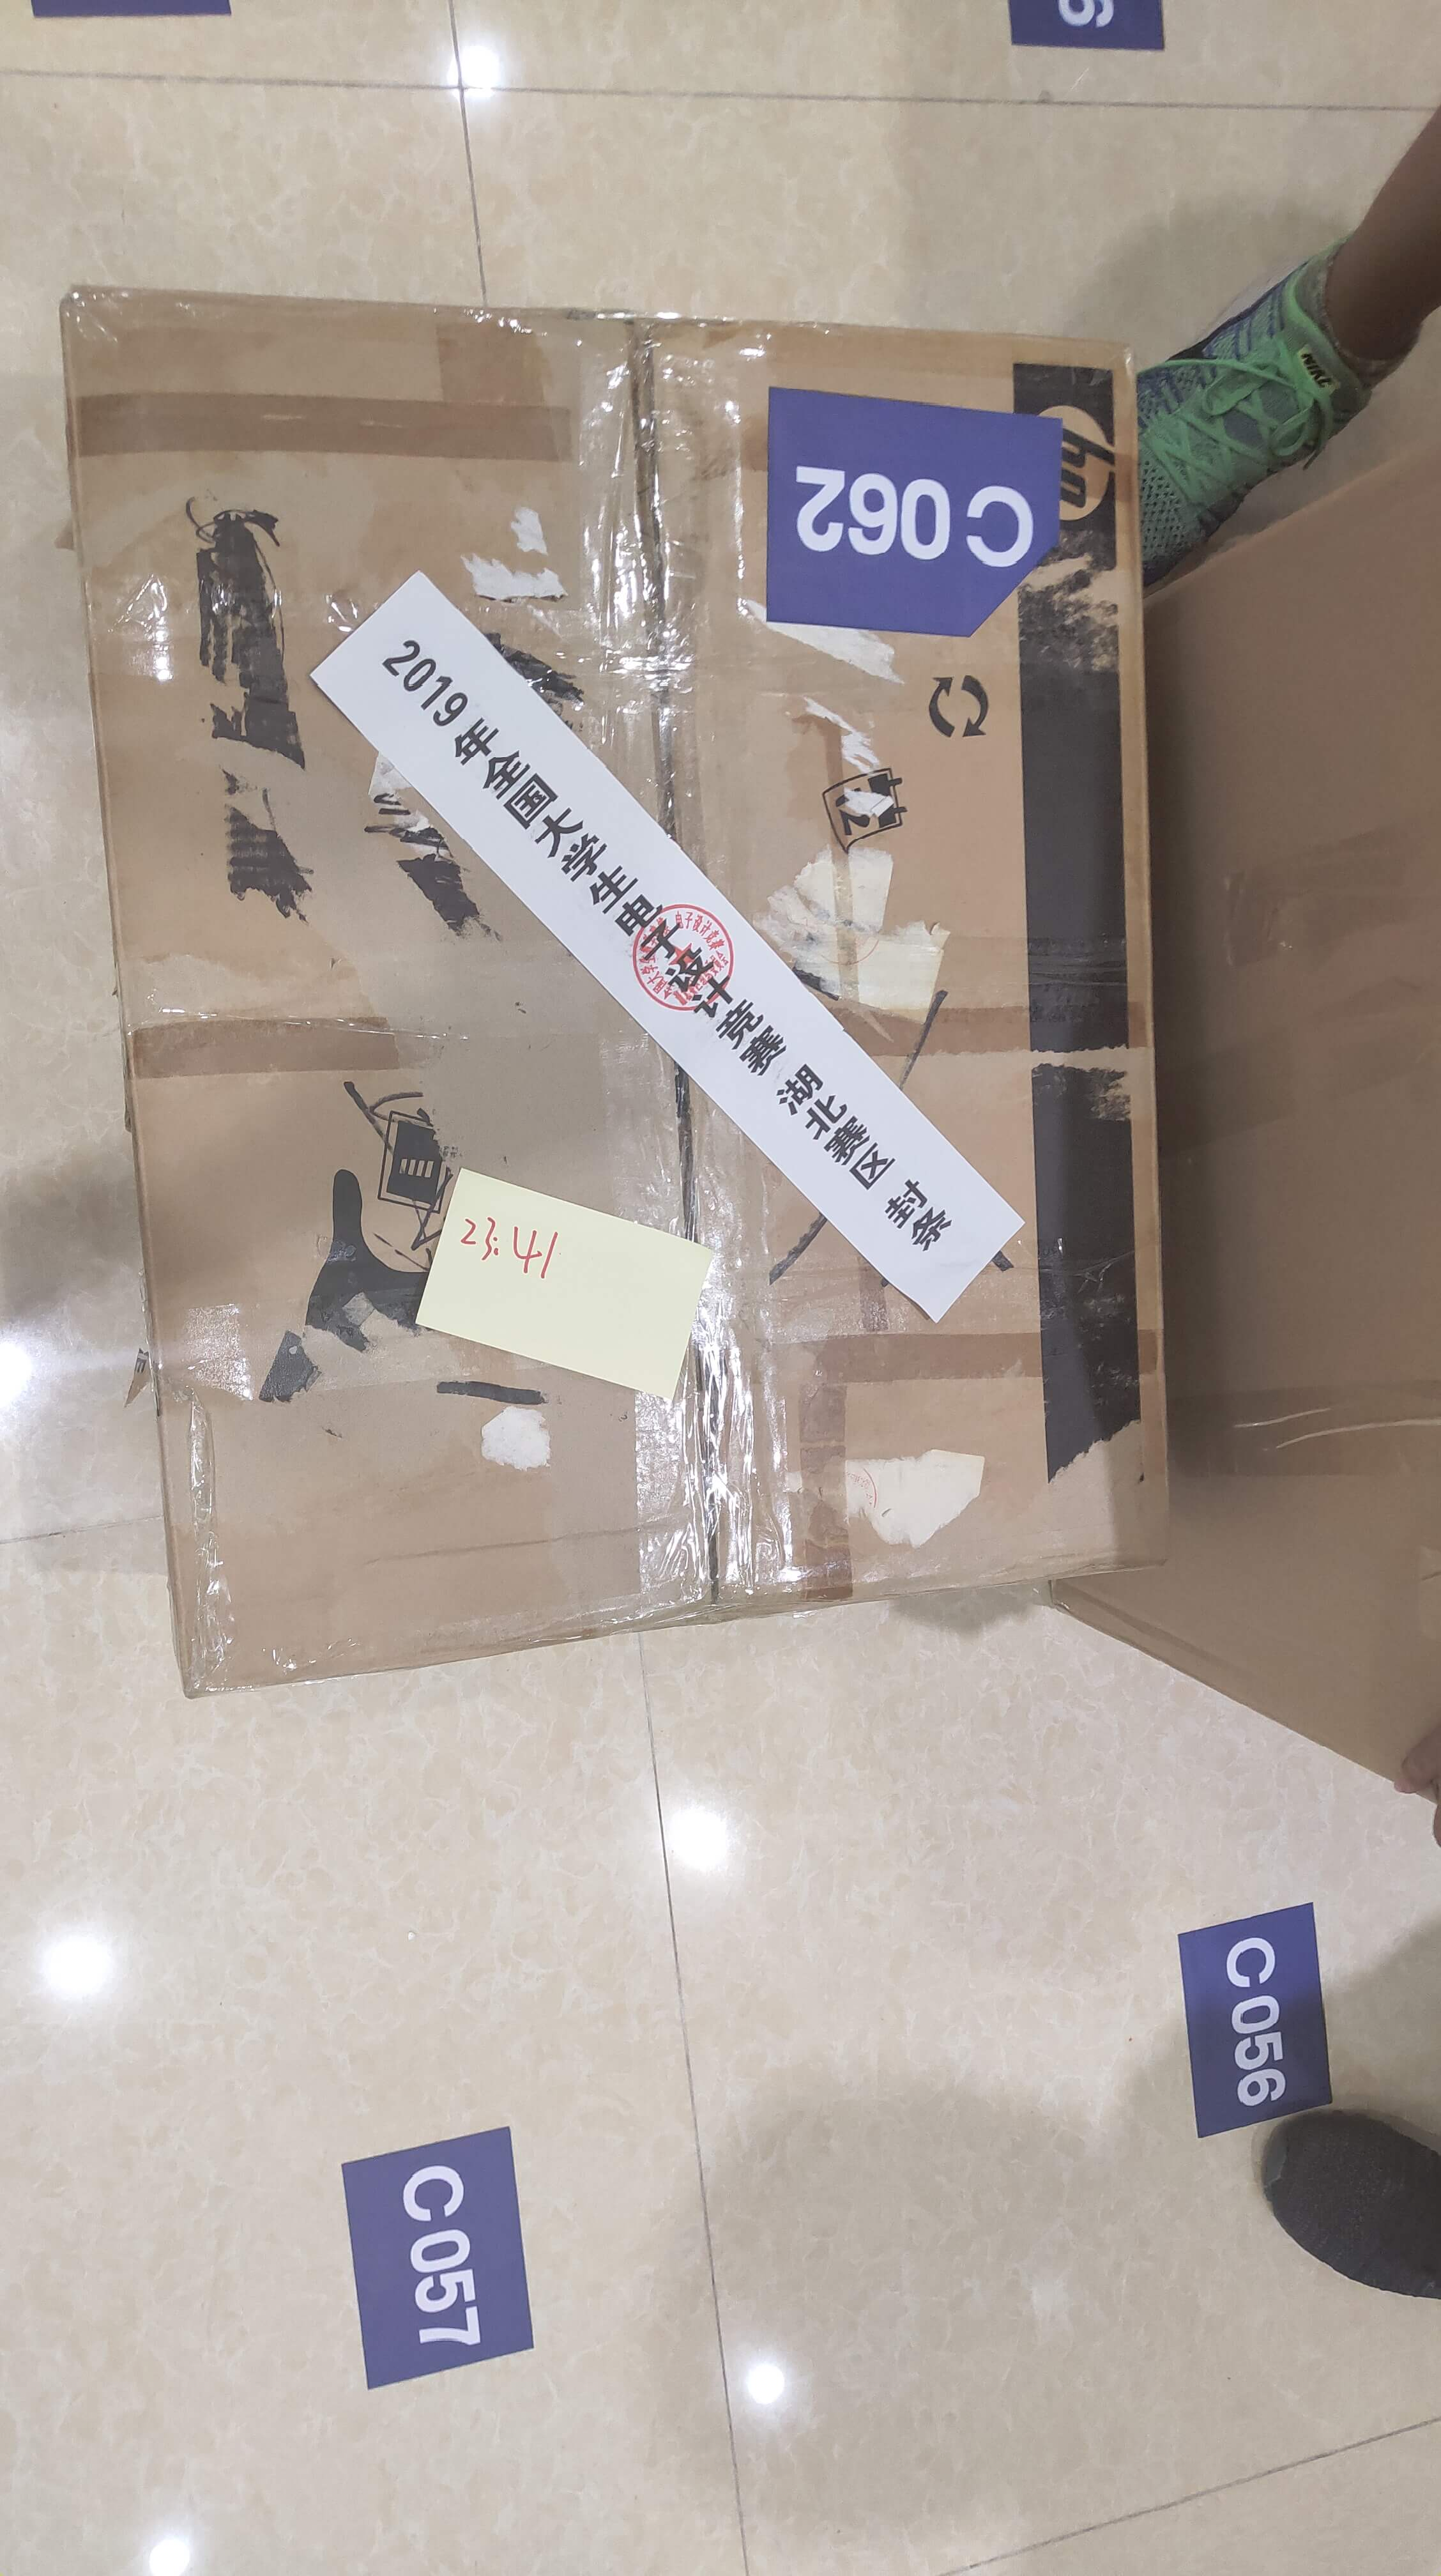
\includegraphics[width=1.0\textwidth]{me8.jpg}
	\caption{送至武汉大学 \label{fig:scatter}}
\end{figure}

\chapter{ 杂谈 }

这个部分,则是对大学这两年避不开的话题谈谈自己的经历及看法。还是那句话,如有错误,欢迎指正,如有帮助,不胜荣幸!

\section{读研}

对于这个议题,我的看法是“不要人云亦云,有自己独立的思考”。我想我自己可能没有资格谈论这个话题,因为我也不是过来人。所以我摘录laike9m的一篇《所以,到底要不要读研?》希望对大家有帮助:


过去几年,我零散地表达过一些对读研的看法。鉴于最近有人感兴趣,我也正好写篇文章总结一下。本文所说的“读研”,特指在中国境内读三年制硕士研究生。这也符合大多数人的情况。本文所谈论的“读研”不包括:读博、读两年制项目、在职研究生、出国读书等等。

我对读研怎么看?用一句话概括就是:\textbf{如果你明确知道读研就是达到既定目标过程中所缺失的那个条件,那就去读。否则不要读。}
	
在展开讨论之前,我必须先讲一个致命的思维盲区:\textbf{权衡要不要做某件事的时候,只看到做这件事的收益,而完全不考虑因此导致无法做别的事所造成的损失}。以读研为例。有人说“读研提升了学历,增加了进大企业的机会,好处太多了,一定要读”。True,我承认有这些好处。问题是,你把这些好处放在天平的一端,另一端放什么?如果什么都不放,那最后的结论当然是读研好。但应该这样比吗?不该啊。要放在天平另一端作为比较对象的,不是三年前的你,而是没读研去做了其它事的那个你。一个人\textbf{要判断的,不是读研带来了多少收益,而是读研和其它选择哪个收益更大}。这才是正确的思考方式。	
	
有了上面这些基础,我们来列举几种常见的值得读研的情形。

情形一,你想去的地方,对学历有明确要求。包括但不限于积分落户、某些事业编制、男/女朋友的家人要求你必须是硕士等。没什么好说的,去读就行了,毕竟你没法改变规则。

情形二,你想去的地方,对学校有明确要求。比如某岗位要求必须是 211 及以上,而你之前只是普通一本。这条看似和上一条类似,但其实不一样,后面会说。

情形三,你想转行。比如误入了天坑专业的学子,想完全依靠自己力量跳出去实在是太难了。用人单位看到你本科专业,可能直接就把简历扔了。去读个对口专业的研究生会好很多。

情形四,你想去的地方,拥有硕士学历能带来更好的发展。诸如政府机关、国企、军队,唯学历论依然盛行,本科生和硕士可能会被分配完全不同的就职岗位和培养路径。

当然,上面只是几个例子,无法涵盖全部情况。归纳起来还是最开始说的:如果你明确知道读研就是达到既定目标过程中所缺失的那个条件,那就去读。

然而,大部分人连目标都不确定,只不过是把读研当做一种改变命运的美好幻想罢了。幻想的形式包括但不限于:

\begin{enumerate}
\item 谁说计算机从业人员就只有程序员、进公司 code 这一条路了,选择读研读博继续深造的,可能是想在计算机前沿领域进行研究,以后仍然可以选择进公司或者出国留学然后留校留研究院搞科研学术。	

\begin{lstlisting}
读博我们这里不谈,但你跟我讲读研深造?我就想知道第一年上课最后一年写毕业论文找工作可能还有实习请问你要怎么搞研究?把学术界当儿戏以为成果能随便就能出?你想读研留校搞学术,我还想去二次元开后宫呢,好不好?
\end{lstlisting}

\item 因为你儿子 /女儿以后可以跟同学说我爸不是个纯 code 屌

\begin{lstlisting}
笑尿了,读研就不是“纯 coder”,就高大上了。这种话简直不值一驳,能说出这话的人可以想象是处在怎样一种封闭无知的圈子里。
\end{lstlisting}

\item 控制变量,能力相等的情况下,有研究生学历的你,和没有研究生学历的你,哪个在别人眼中更优秀?

\begin{lstlisting}
这个还是有必要说一下。对于能提升学校档次的考研,我完全支持,但首先你得确定这是你需要的,其次是你得去一个真正提升了档次的学校。你说我从xx理工学院城市学院考研到xx化工学院科亚学院,读不读又有什么区别呢?还不如去积累工作经验。
\end{lstlisting}

\item 看看今年研究生算法岗的神仙打架和工资....

\begin{lstlisting}
不好意思,我就没见到哪家公司的岗位指定了要研究生,因为他们知道学位不等于能力,一个 NB 的本科生可以顶十个水货硕士。
\end{lstlisting}

\item 能考上研究生的,整体水平要比本科水平高。不要把公司当傻子,研究生这个门槛天生就隔绝了能力水平稍低的人。

\begin{lstlisting}
不值一驳。
\end{lstlisting}

\item 因为太菜了,纯写代码竞争不过各位大佬。

\begin{lstlisting}
所以你读完研就不菜了?读研不能让你脱胎换骨变成另一个人,醒醒吧。
\end{lstlisting}

\item 大部分人平庸到谈不上靠能力争取到话语权,所以只能尽力找一个块儿厚点的敲门砖。

\begin{lstlisting}
这句话不能说没道理,但首先,你总得先选好想进的门吧?
\end{lstlisting}

\item 可能你眼中的程序员只是日常 CRUD 吧

\begin{lstlisting}
嗯,研究生牛逼,做的都是高大上的工作,CRUD 什么的太没技术含量啦。
\end{lstlisting}

\item 样本虽然小,但是我身边确实就学历和经验来看,学历高的比经验足的后劲更大。前几个月刚毕业来公司的交大小伙,现在熟悉业务了代码写得嗖嗖的,又好又快,而且产品那边一些新需求他也能就着英文文档去啃出来。而另一位 3 年经验的专科同事,虽然解决问题挺熟练,但是文档几乎不会啃,全靠简书和 csdn 里面的博客对着写,有些生僻点的玩意百度找不到,他那边就 gg 了,更不用说数据处理,除了日常的增删改查,其他的复杂的数据处理他那边就会僵住.

\begin{lstlisting}
您厉害,这变量控制得真好。他厉害不是因为他是研究生,是因为他是交大的啊。
\end{lstlisting}

\item 作为一名研究生应届毕业生,来说说我对此问题的看法 1.研究生选择更多。可以选择去做科研,做教师,工作职位可选择的也多,比如女生不想做研发可以做测试等等 2.发展空间更大。个人认为学历还是很重要的,尤其是在以后职位的晋升上 3.思维方式和学习更力。研究生期间,学习到更多的应该是看问题的方式,对行业的见解等等,而不仅仅是码代码 4.起点更高。更容易去大公司,起薪也会更高

\begin{lstlisting}
1 不说了。2 是一种很奇怪的误解,因为我发现老一辈人(比如我妈)真的会这么想。但实际上除了少数地方比如国企,大部分工作并不存在本科生发展空间受限一说,尤其当你讨论的还是 CS 专业的时候。3 有一定道理。4 我要重点反驳一下,这就是前面提到的思维盲区的典型。研究生的你,的确更有可能拿到比本科的你更好的 offer。然而,和工作了三年的你相比呢?三年时间,快的话可以涨薪两次或是跳槽两次了,在大公司的话升一级没问题,快的话可以升两级,更不要提工作经验的积累了。别忘了学校和公司可是完全不同的。
\end{lstlisting}

\item 程序员只是青春饭,你会发现上了年纪就不行了

\begin{lstlisting}
读研之后你老了三岁,能吃这口饭的时间更少了。
\end{lstlisting}

\item 校招大厂来面试的大多数是研究生,足以说明问题

\begin{lstlisting}
看来 Google 不是大厂了。再说进了公司你就会发现研究生和本科生干活真的没什么差别。
\end{lstlisting}
	
\end{enumerate}	

这些幻想要批判起来说一年也说不完。不过相信大家也发现了一些共性,就是这种盲目推崇读研的人,往往对很多问题都缺乏基本了解,看问题也非常片面。我暗自揣测,他们中大部分可能并没有真正读过研究生,却又把自己目前的不如意归咎于没有读研,并幻想出了所谓读研之后的美好生活。我在计算所的时候,周围很多同学都觉得读研浪费时间,也包括我在内。有个哥们实在受不了实验室安排的无聊工作直接退学然后面试进了头条,人家也没嫌他学历不够。总之呢,读研这件事好不好,各人有各人的情况。对想进互联网行业的同学,可能确实是浪费时间,但若是想去考公务员或者拿户口,可能又很必要。关键还是要清楚自己的目标,分析自身情况,再来判断读研到底是不是一个好的选择。

写这么多,想说的基本都说了。我试图保持客观,但也并不想掩饰对读研的负面看法。说真的,如果国内的研究生学制也是像国外那样是一年或者一年半,我断然是不会写这些的,因为读了也就读了。然而,它是三年,还是你人生中非常宝贵的三年。三年时间是真的不短啊。好好思考一下三年你能做什么,是否值得用这段时间去换一张文凭。我希望所有人都能做出令自己不后悔的选择。

以上就是文章的全部,既然我没有资格谈自己的看法,那我就讲讲自己的一个经历好了。我记的在大二的上学期,那时候是秋招的时间。思科公司来我们学校招聘,招聘的教室就在我们实验室的旁边,思科的某位领导可能是来早了,到处逛逛,就进了我们的实验室。在闲谈中长者就提到了:“我们公司招聘不会把学历放在第一位,更看重个人能力,本科生中也有很多能力强的。在中国的学术环境的影响下,读研并没有起到应有的作用”。

\begin{figure}[htbp]
	\centering
	
\includegraphics[width=\textwidth]{travel2.jpeg}
	\caption{ 神农架之行 }
\end{figure}

\section{终生学习}
好吧,还是要继续摘录其他人的文章了。先带大家看一篇Summer所写的《 每一个编程从业者都应该是「终身编程者」 》:

\textbf{程序员是很棒的职业}

世界是由软件构成的,而程序员是撰写软件的人。

在未来,很多职位会消失,这是因为计算机和软件可以取代它们。但是从另一个角度看,因为我们需要不断开发和维护这些程序,所以这么一想,程序员的前景还是很美好的。

即便你不把编程当成职业,也可以拿编程来解决生活中的问题,以工程师的思维来思考这个世界,并尝试去优化自己的生活。

\textbf{编程是一辈子的}

从决定把编程作为职业开始,我就告诉自己,编程应该搞一辈子。为啥?因为这个职业对经验和学习能力要求太高了,隔语言如隔行,得无时不刻地学习,没有经验还找不到工作。如果决心不够坚定,自己肯定会很难混下去。所以只要入这个行,不管十年后是否从事编程的工作,编码都应该是一辈子的。

有了这个定位,就不怕自己学的东西太广太泛了,脑子里会想:「我这是在打地基」。遇到编程问题时,也会去寻找最佳实践,会带着长久发展的思维去思考。例如说不把自己的专业当成 PHP Web 开发 ,而是 计算机科学,会主动去学习 软件工程。

把编程当成终身职业时,工作也会变成学习进步的途径,而不是艰苦地讨生活。业余时间用来学习和编码,也会变得名正言顺。随着而来的好处是,同样几年过去了,你比身边的同事要经验丰富得多。

上面的文章是来自learnku社区站长的一篇文章。一入编程深似海,不断学习成必然。就笔者写作的年代来看,是处于技术不断革新,基本上每月都有新的技术、新的概念提出来,意味着程序员学习的东西不断的累加。但是就目前的趋势来看,现在的开发都讲究自适应,也就是一套代码在各大平台都能完美的运行。这样自然是大大减少了程序员的学习成本。也许未来能出现一统多端的语言,可能是Dart也可能是JavaScript,也可能是其他的。


\section{奖学金}

首先努力之后获得成绩是值得肯定的。我们学校的奖学金的有很多,同时制度也相对健全,只要满足要求就能申请。我也通过自己的努力凭大一的成绩获得了奖学金。但是我持有以下观点“努力学习是为了追求卓越,奖学金只是在追求卓越路上的小小的奖励”。

\section{论坛}
我是一个喜欢逛论坛的人。刚上大学的时候接触到的两个论坛:知乎、CSDN。现在都不怎么逛了,首先知乎上通常是长篇大论读起来太费劲,其次自己没达到知乎的平均水平-动不动就是《 月薪5W是一种怎样的体验》 ,最后知乎并不是技术性的论坛。对于CSDN我认为他的技术文章参差不齐,且种类繁多,所以我一种把它当作查资料的工具在用。

现在我逛的论坛有很多,下面给大家做推荐( 软件学习相关 ) :

\begin{enumerate}
\item GitHub:\href{https://github.com/}{https://github.com/} 

全球最大的同性交友平台,优秀的代码托管平台。
	
\item 掘金:\href{https://juejin.im/}{https://juejin.im/} 

文章质量高!针对性性强。

\item V2EX:\href{https://www.v2ex.com/}{https://www.v2ex.com/} 

这个论坛没有太多技术性的文章。喜欢它的原因有两个:“酷工作”板块十分活跃,在这个版块下可以看到公司的招聘需求,也可以看到并下载其他人的简历。其次它更像是程序员的休闲灌水群。

\item SegmentFault: \href{https://segmentfault.com/}{https://segmentfault.com/} 

有着中国的StrakOverFlow之称,是一个问答性质的平台。同时思否学院中的课程质量较高。

\end{enumerate}	
此外还有learnKu、简书等优秀的平台。


\begin{figure}[htbp]
	\centering
	
\includegraphics[width=0.6 \textwidth]{me2.jpg}
	\caption{ 发际线 \label{fig:scatter}}
\end{figure}

\section{竞赛}

大学里面的竞赛有很多,电子设计大赛只是其中之一。但是并不是每一个都适合你参加,所以择其善者而攻之。想参加比赛不要着急,首先你要有技术的积累,只有你自身实力够强,老师才愿意带你,同学才愿意找你。准备比赛的时间应从进校就开始,但是参加比赛的时间应该是大二下的寒假才开始。当你进入大二下,你就是学校参加比赛的主力选手了。以下我只介绍几个我所了解的:

那年寒假有“全国大学生创新创业训练计划”的申报,注意不是比赛,只要完成最后的答辩结题即可,且通过概率极高。大家一定要把握好这个机会。这个比赛能获得保研加分,但是不具有保研资格。想要获取保研资格还需通过学生手册上列举的比赛。

然后大二暑假就有“全国大学生电子设计大赛”,这个比赛在信息学院和机电学院参与的人数很多,比赛的方向也很多。需要找好队员,和选好参赛方向。电子设计大赛总的来说分为五类:“电源类”、“测控类”、“信号类”、“高频类”、“无人机”。其中参与人数最多的就是“电源类”与“信号类”。无论是那一类都不简单,都需要做好长期奋斗的准备。

在大三的要参加准备以久的“挑战杯”和“节能减排”了,这可是竞赛里面的两大巨头。做好了你就不用努力了,做不好你可能“人财两空”。之所以说“准备以久”,意味着这个项目一定是经过长时间的孵化,并且经历过许许多多的答辩历练。在我写下这篇文章的时候,这两个比赛都还在继续推进。我这一年的“挑战杯”是创业类的比赛,也就是“小挑”。这对我们信息学院的学生并不是十分有利,但是我们都在尽力做,并且对自己有信心。

\begin{figure}[htbp]
	\centering
	
\includegraphics[width=\textwidth]{me3.jpeg}
	\caption{ i创杯 }
\end{figure}

我的看法就是所有比赛的选题还是要有老师的指导比较好,最好是老师正在研究的课题。所以,在此再次感谢所有帮助过我的老师。

\section{社团}

最后一个话题,我选择留给协会。

此前我一直有个遗憾,就是自己没能加入一个小团体的社团,面试啥啥失败。但是,“电子科技协会会长”的身份就像一份礼物一样摆在了我的面前。

这段往事有点不堪,但是我还是想把它写出来。在我的上一届,我认为是做的不够好的,糟糕到换届的时候从头至尾找不到人竞选。我有个很强势的女同学,是其中的干部,也是原本的会长候选人。她在换届的前一天找到我,想让我担任副会长,我充满疑惑的接受了。也在同一天晚上,“协会会长”这份礼物就送到了我的面前,既然大家都不想干那我就干。

我当会长的第一年是从2018年暑假开始的。先自我评价一下这一年,“很烂,承诺的事情没做到”。毕竟是第一次当会长,既没有示范,也没有实习。当时我承诺的是一个学年将举办4次活动,也只举行了一次,会员大会啥的都没有。因为我陷入了一个巴掌拍不响的局面。

协会又混混噩噩到了换届的时候,此时我大可拍拍屁股走人,大不了被别人背后小声的骂几句。但是我是不甘心的,我有野心要把协会做好,要做到五星级社团。于是我选择再干一年,如果干不好那就再干一年。此时,我不在是一个人奋斗,我有了一群志同道合的伙伴。那么这一年,我要为协会未来5年的发展奠定基础,没有的东西我们从头建设,已有的东西发扬传承。

这里我想说明一下,这是我的个人文章为什么要已协会的名义发表呢?我想我把电子科技协会当成了自己的家,家是付出而不是索取,同时我也想这个家能留下我的印记。

\emph{电子科技协会,在奔跑。}

\begin{figure}[htbp]
	\centering
	
\includegraphics[width=\textwidth]{logo.jpg}
\end{figure}

\end{document}
